\documentclass[12pt,openany]{book}

%%  Dimensions and URL
\usepackage[margin=1in]{geometry}
%\usepackage[hyperindex]{hyperref}

\usepackage{amsmath,amssymb,amsthm,bm}
\usepackage{graphics,epsfig,psfrag}
\usepackage{makeidx}

\newtheorem{theorem}{Theorem}
\newtheorem{proposition}{Proposition}
\newtheorem{lemma}{Lemma}
\newtheorem{corollary}[theorem]{Corollary}
\newtheorem{definition}{Definition}
\newtheorem{example}{Example}
\newtheorem{fact}[theorem]{Fact}
\newtheorem{problem}[theorem]{P}
\newtheorem{solution}[theorem]{S}



\newcommand{\vecnot}{\underline}


\newcommand{\SetIn}{\ensuremath{\mathrm{1\!\!1}}}
\newcommand{\Expect}{\ensuremath{\mathrm{E}}}
\newcommand{\Var}{\ensuremath{\mathrm{Var}}}

\newcommand{\RealNumbers}{\mathbb{R}}
\newcommand{\RationalNumbers}{\mathbb{Q}}
\newcommand{\Integers}{\mathbb{Z}}
\newcommand{\NaturalNumbers}{\mathbb{N}}
\newcommand{\IndexSet}{\mathbb{I}}
\newcommand{\JndexSet}{\mathbb{J}}
\newcommand{\Complement}{\mathrm{c}}
\newcommand{\IndicatorFcn}{\mathbf{1}}
\newcommand{\Trace}{\mathrm{tr}}


\newcommand{\decreg}[2]{\overset{#1}{ \underset{#2}{\gtrless} }}

%% Definitions
%%
\renewcommand{\baselinestretch}{1.25}
\newcommand{\defn}[2]{\textbf{\textrm{#2}}\index{#1!#2}}

%% Definitions
%%
\renewcommand{\baselinestretch}{1.25}

\makeindex

\begin{document}

\author{Jean-Francois Chamberlan}
\title{
\Huge{An Introduction to Detection and Estimation}\\[5mm]
\Large{Class Notes for\\Engineering Students}}

\frontmatter
\maketitle

%\chapter*{Copyright}
%Copyright \copyright\ 2006--2009
% The FRED Project \\
%Jean-Francois Chamberland

%Permission is granted to copy, distribute and/or modify this document under the terms of the \emph{GNU Free Documentation License}, Version 1.2 or any later version published by the \emph{Free Software Foundation}; with no Invariant Sections, no Front-Cover Texts, and no Back-Cover Texts.
%A copy of the license is included in the section entitled ``GNU Free Documentation License''.

%\tableofcontents

%\frontmatter
%\chapter{Preface}

These notes provide an introduction to probability.
It presents a treatment of probability concepts and techniques necessary for a basic understanding of the subject.
The notes are designed to be used in a semester course totaling 45 hours.
The reader is expected to have a basic understanding of calculus including sequences, series, derivatives and integrals.

Possessing some programming skills will also help in order to appreciate and use the computing material and examples contained in the text.
Probability theory makes predictions about experiments whose outcomes depend upon chance.
Consequently, it lends itself beautifully to the use of computers as a tool to simulate and analyze experiments.
The computer is a powerful aid in understanding basic results of probability theory, especially through imaging and graphical representation of difficult concepts.
Finally, computer programs are useful in solving problems that do not lend themselves to close-form expressions.



\mainmatter

%\chapter{Digital Communications}
\label{chapter:DigitalComm}

The term \emph{digital communications} broadly refers to the transmission of information using digital messages or bit streams.
There are notable advantages to transmitting data  using discrete messages.
It allows for enhanced signal processing and quality control.
In particular, errors caused by noise and interference can be detected and corrected systematically.
Digital communications also make the networking of heterogeneous systems possible, with the Internet being the most obvious such example.
These advantages, and many more, explain the widespread adoption and constantly increasing popularity of digital communication systems.


\section{System Components}

A typical digital communication system can be represented by the functional block diagram depicted in Figure~\ref{figure:BlockDiagram}.
It is composed of five basic components.
The input block contains the source, which produces data (such as voice, emails, or images), and it also includes all the operations that are required to convert the original signal waveform into a format suitable for transmission.
The transmitter takes bits from the input block and sends them over a channel using electromagnetic signals, or some alternate means.
Communication channels come in many flavors.
For instance, a transmission can take place over an ethernet cable, a coaxial cable, or free space (wireless communications).
There are also more esoteric channels like a hard drive platter, a compact disc, or a memory stick.
The role of the receiver is to recover the sent message from a collection of measurements.
This unit may need to extract the signal from noise and, possibly, correct errors that may have occurred during transmission.
Finally, the output block takes the received information and puts it back into a format that is appropriate for the end-users.

\begin{figure}[htbp]
\begin{center}
\begin{psfrags}
\psfrag{I}[c]{Input}
\psfrag{O}[c]{Output}
\psfrag{T}[c]{Transmitter}
\psfrag{R}[c]{Receiver}
\psfrag{C}[c]{Channel}
\epsfig{file=Figures/diagram,width=98.7mm}
\end{psfrags}
\end{center}
\caption{A digital communication system contains five basic components.
These building blocks appear in this diagram.}
\label{figure:BlockDiagram}
\end{figure}

Figure~\ref{figure:BlockDiagram} also alludes to the natural symmetry present in digital communication systems.
Operations that take place on the transmitter side must often be undone at the destination.
As such, complementary steps are frequently studied in pairs.
Our treatment of digital communications follows this general approach.


\subsection{The Input-Output Blocks}

The role of the input block is to take information in its natural form and to convert it into a digital format.
Depending on the nature of the source, two operations may be necessary to digitize the information waveform.
\emph{Sampling} is a signal processing technique that transforms a continuous-time function to a discrete-time signal.
The conversion of a sound wave into a sequence of samples is a common application of sampling.
The second action that may be needed is \emph{quantization}, which maps a continuous-space signal into a discrete set of possible values.
The combination of these two operations will transform an analog signal into a digital message.

\begin{figure}[htbp]
\begin{center}
\begin{psfrags}
\psfrag{I}[c]{Input}
\psfrag{S}[c]{Sampling}
\psfrag{Q}[c]{Quantization}
\psfrag{E}[c]{Compression}
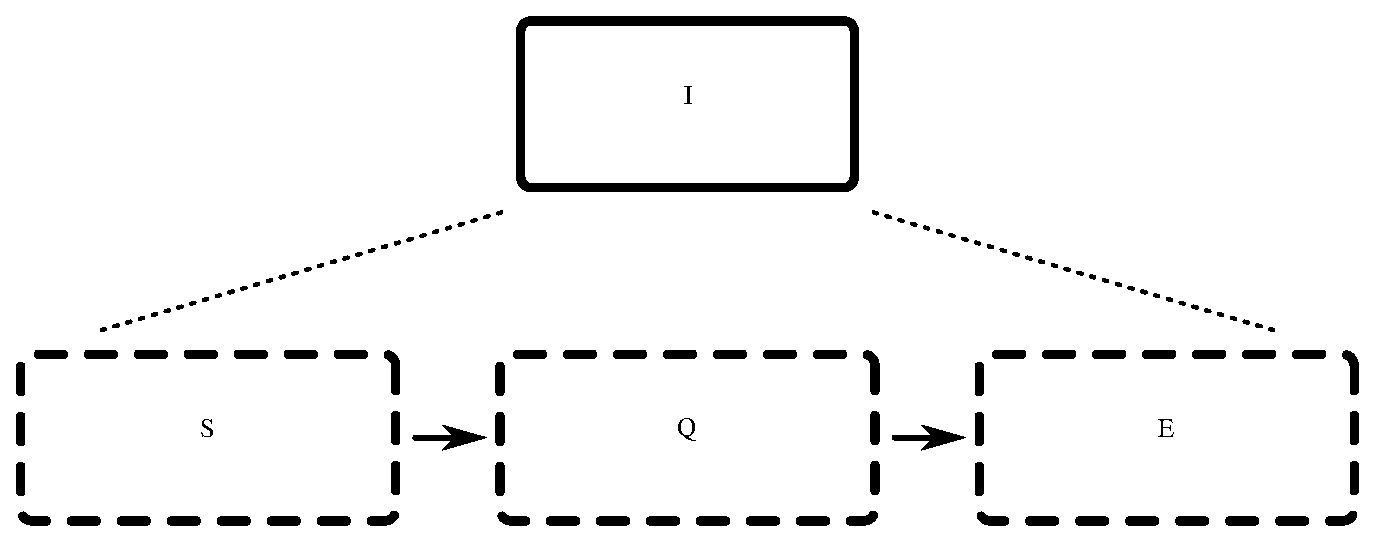
\epsfig{file=Figures/input,width=112.7mm}
\end{psfrags}
\end{center}
\caption{The input block can be further divided into three operations: sampling, quantization and data compression.
The first two operations are necessary to transform an analog waveform into a digital signal; whereas the last block is optional and provides a means to reduce the size of a digitized message.}
\label{figure:BlockInput}
\end{figure}

The optional step of \emph{data compression}, or source coding, is often employed at the origin to reduce the size of the message to be transmitted.
This, in turn, brings down the consumption of expensive resources such as power, spectral bandwidth and hard disk space.
On the downside, data processing entails additional computations and delay, and the compressed data must be expanded before being accessed.
This involves using extra processing on the receiver side as well.
Some compression schemes reduce the quality of the data.
These schemes usually feature better compression ratios at the expense of introducing small variations in the data.
The MPEG standards, including the MP3 audio layer, provide examples of lossy compression schemes.

\begin{figure}[htbp]
\begin{center}
\begin{psfrags}
\psfrag{O}[c]{Output}
\psfrag{I}[c]{Interpolation}
\psfrag{R}[c]{Reconstruction}
\psfrag{D}[c]{Decompression}
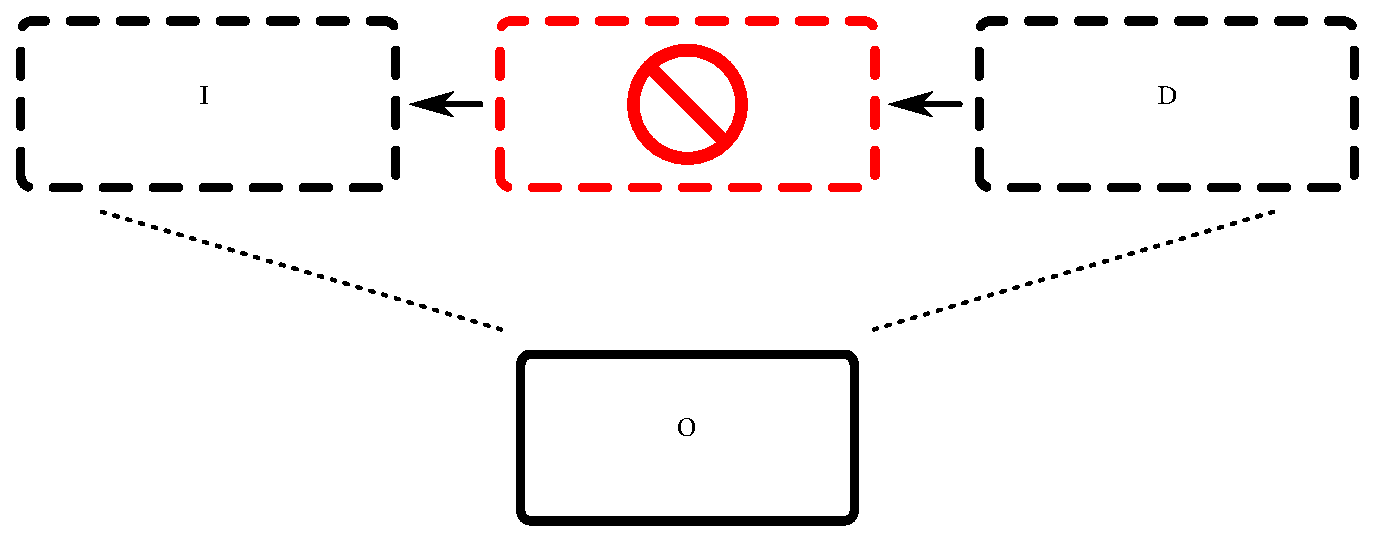
\epsfig{file=Figures/output,width=112.7mm}
\end{psfrags}
\end{center}
\caption{The operations executed at the transmitter must typically be undone at the destination.
When passed through the output block, the received data is first decompressed and put in a format that suitable for signal processing.
Furthermore, an analog signal must be reconstructed from the sampled data point.
While these two steps can reversed without any loss, the quantization step cannot.
This is because quantization loses a small part of the original information.
Instead, the reconstruction step reverses quantization step in an approximate way to minimize the distortion.}
\label{figure:BlockOutput}
\end{figure}

At the output of the system, the data must be transformed back into a format that is acceptable to the end-user.
The received message must be decompressed.
Note that for the destination to be able to recover the original data, it must understand the encoding scheme utilized by the sender.
In other words, the decoding method must be known at the receiver.
If the original signal is a continuous-time waveform, then an interpolator can be used to reconstruct the waveform from its sample values.
The quantization block present at the input does not have an exact counterpart at the output.
This deficiency follows from the fact that quantization cannot be perfectly undone because information is typically lost when a continuous-valued signal is discretized.
The level of \emph{distortion} associated with quantization can, however, be controlled by choosing an appropriate quantizer and reconstructing the signal in a sensible way.
In most cases, the impact of quantization is minimal.


\subsection{The Transmitter-Receiver Pair}

A channel code is used at the transmitter to shield data sent over the channel against errors due to noise and interference.
This level of protection is achieved by adding redundancy to the information bits in a structured manner.
Audio compact discs make use of a \emph{Reed-Solomon code} to protect digital music from scratches and dust, whereas a low-latency \emph{convolutional code} is employed in cellphones to carry voice signals.
The second task of the transmission unit is to modulate the digital bit-stream onto an analog carrier prior to transmission.
The possible waveforms emitted by the transmitter are chosen from a finite number of symbols.
The transmitter must produce a signal that remains confined to its assigned spectral bandwidth.

\begin{figure}[htbp]
\begin{center}
\begin{psfrags}
\psfrag{T}[c]{Transmitter}
\psfrag{E}[c]{Encoder}
\psfrag{M}[c]{Modulation}
\epsfig{file=Figures/transmitter,width=72.45mm}
\end{psfrags}
\end{center}
\caption{At the transmitter, redundancy is added to the digital message to protect information bits against noise and interference.
Once this is completed, the bit stream is modulated onto an analog carrier and transmitted to the destination.}
\label{figure:BlockTransmitter}
\end{figure}

The message then propagates through the communication channel.
This is the physical medium that bridges the gap between the transmitter and the receiver.
In most applications, the channel acts as to transfer the data to a different place.
However, in hard disk drives and compact discs, the information is stored simply to be accessible at a later time.
Most communication channels cause signal degradation.
The message may be subject to attenuation, interference and noise corruption.
The communication channel may be unreliable; and its environment, hard to characterize.
Recovering the original data from a set of measurements available at the receiver is one of the many challenges of digital communication systems.

\begin{figure}[htbp]
\begin{center}
\begin{psfrags}
\psfrag{R}[c]{Receiver}
\psfrag{M}[c]{Demodulation}
\psfrag{D}[c]{Decoder}
\epsfig{file=Figures/receiver,width=72.45mm}
\end{psfrags}
\end{center}
\caption{On the receiver side, the sent symbols are extracted from the received signal.
Error-correction techniques are then applied to insure the integrity of the acquired data.
Finally, the digital message is restored to its original format.}
\label{figure:BlockReceiver}
\end{figure}

The receiver is tasked with extracting the original symbols from noisy measurements.
The first step consists of estimating which symbols were sent by the transmitter over the channel.
This procedure is termed \emph{demodulation}.
These symbol estimates are then translated back into information bits by the decoder.
Redundancy is removed from the data, and the original format of the information bits is restored.
If the channel conditions are harsh and the local measurement too noisy, then this process fails and the corresponding data is lost.
Scratching a compact disc repetitively will illustrate this point well.
After substantial disc abuse, a player is no longer able to reconstruct the music.


\section{Common Channels and Applications}

Various communication channels can provide a connection between a transmitter and its destination.
Common wireline channels include coaxial cables, ethernet cables, and twisted-pair wires.
Optical fiber offers a high-capacity solution for heavy applications.
Compact discs and DVDs are also based on optics and they can be employed to store information on discs.
Finally, wireless electromagnetic channels are popular for their convenience and broadcast capabilities.

Digital communication occupies a central role in almost every aspect of contemporary life.
Most businesses rely directly or indirectly on networked computers and the Internet for day-to-day operations, and digital technologies have become a staple of the entertainment industry.
Below, we provide a few examples of digital communication systems that you may be familiar with.

\paragraph{Cable Modem:}
A cable modem enables point-to-point communication over the cable television infrastructure.
They are primarily employed to deliver broadband Internet access, taking advantage of unused bandwidth on a cable television network.
With the advent of voice over Internet protocol (VoIP) telephony, cable modems can also be used to provide telephone service.

\paragraph{Wi-Fi Technology:}
Wi-Fi is a global set of standards that allows wireless inter-networking.
In particular, it includes the IEEE 802.11 protocol suite (e.g., 802.11b, 802.11g and 802.11n).
Wireless access points, also called \emph{hotspots}, often provide users access to the Internet.
Wi-Fi products can be used as an enabling technology for \emph{mesh networks}, which offer connectivity to large urban communities.

\paragraph{Bluetooth:}
Bluetooth is a wireless protocol designed for short-range communication, and it is used primarily to create personal area networks.
Bluetooth provides a means to exchange information between such devices such as mobile phones, personal computers, digital cameras, and a myriad of accessories.

\paragraph{Hard Disk Drive:}
A hard disk drive is a non-volatile storage device that stores digitally encoded data on rapidly rotating platters with magnetic surfaces.
Today, hard drives can be found in computers, digital audio players, personal digital assistants, game consoles and other embedded computing devices.
Data on a hard disk drive is recorded by magnetizing ferromagnetic material directionally, and is read back by detecting the magnetization of the material.

\paragraph{Compact Disc:}
The compact disc (CD) is an optical disc used to store digital data, and remains one of the popular playback media for commercial audio recordings.
A standard compact disc can store approximately 650 Megabytes of data.
The data is stored on the disc as a sequence of bumps that are stamped into the polycarbonate during production.
A reflective layer is added so that the data can be read by using a laser to distinguish between \emph{pits} and \emph{lands}.

In a recordable compact disc (CD-R), a photosensitive dye is used instead.
The write laser of a CD recorder changes the color of the dye to allow a standard CD player to read the data, just as it would with a standard stamped disc.
A re-recordable disc medium (CD-RW) uses a metallic alloy instead of a dye.
The write laser in this case is used to heat and alter the properties of the alloy, and hence change its reflectivity.
A CD-RW does not possess as great a difference in reflectivity as a stamped compact disc, and so many earlier audio players cannot read CD-RW discs, although most later CD audio players and stand-alone DVD players can. 



%\chapter{Detection Theory}
\label{chapter:Detection}

In this chapter, we study hypothesis testing.
A statistical inference problem is termed detection if the attribute set is partitioned into a finite number of subsets and the objective is to identify which of these subsets $\theta$ belongs to.
We refer to the different subsets as hypotheses, and label them as $H_1, H_2, \ldots$
The design problem consists of finding a decision map that takes observation $Y$ as input, and selects one of the possible hypotheses $\{ H_1, \ldots, H_M \}$ as its output.
That is, a detector is a function from observation space $\Gamma$ to the finite set $\{ H_1, \ldots, H_M \}$.

\begin{center}
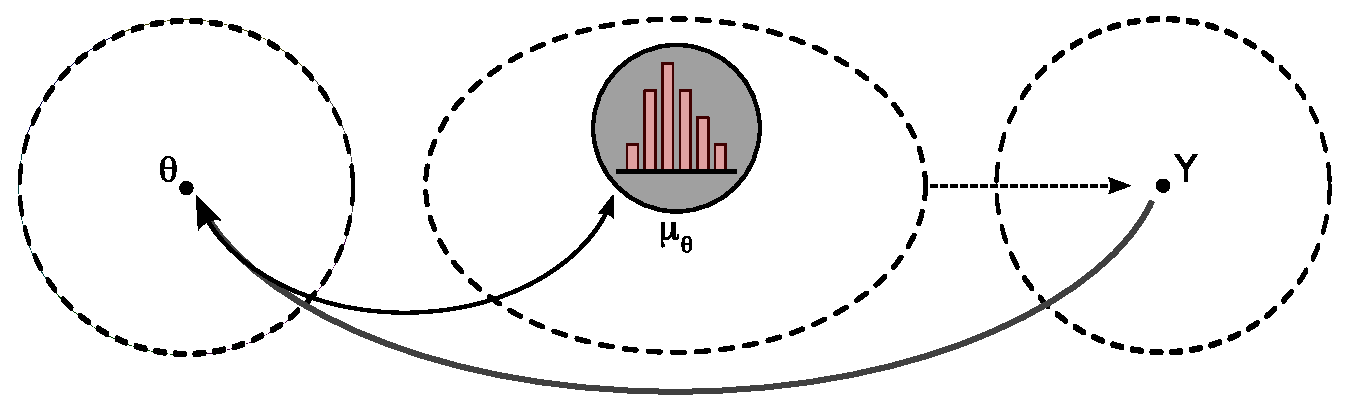
\includegraphics[width=5in]{Figures/2Chapter/HypothesisTesting}
\end{center}

The subset of $U$ that contains parameter $\theta$ is called the \emph{true hypothesis}, which we represent by $H$.
The hypothesis $\hat{H}$ that is selected by observing $Y$ is called the \emph{admitted hypothesis}.
For a specific realization of $Y$, a successful detection occurs whenever $\hat{H}(y) = H$; otherwise, the detector is in error and $\hat{H}(y) \neq H$.


\section{Binary Detection}

In its simplest form, the attribute set contains only two elements.
The goal of the detector is to distinguish between the corresponding two hypotheses.
This scenario is called binary detection.

\begin{center}
\includegraphics[width=5in]{Figures/2Chapter/BinaryDetection}
\end{center}


\section{Bayesian Hypothesis Testing}

We first explore binary hypothesis testing in the Bayesian framework.
The attribute set is assumed to be a probability space with a known distribution.
Specifically, we assume that the true parameter $\theta$ is equal to 0 with probability $\nu(0)$, and it is equal to 1 with probability $\nu(1) = 1 - \nu(0)$.
The probability measure on the elements of $U$ is called the \emph{a priori distribution}, and it represents the knowledge we have about the parameter before getting empirical measurements.

One of the possible performance criteria in the Bayes formulation is to find a detector that minimizes the probability of error.
First consider a deterministic detector of the form $\hat{H}: \Gamma \rightarrow \{ 0, 1 \}$.
Then, the probability of error can be computed as
\begin{equation} \label{equation:ErrorProbabilityDetection}
\begin{split}
P_e &=  \Pr \left( \hat{H}(Y) \neq \theta \right) \\
&= \Pr (\theta = 0 ) \Pr \left( \hat{H}(Y) \neq 0 | \theta = 0 \right)
+ \Pr (\theta = 0 ) \Pr \left( \hat{H}(Y) \neq 1 | \theta = 1 \right) \\
&=  \nu(0) \int_{ \Gamma } \SetIn_{ \Gamma_1 } d\mu_0
+ \nu(1) \int_{ \Gamma } \SetIn_{ \Gamma_0 } d\mu_1 .
\end{split}
\end{equation}
where we use the fact that the binary detector $\hat{H}$ partitions the observation space into two subsets
\begin{align*}
\Gamma_0 &= \left\{ y \in \Gamma : \hat{H} (y) = 0 \right\} \\
\Gamma_1 &= \left\{ y \in \Gamma : \hat{H} (y) = 1 \right\}.
\end{align*}
Using this notation, the probability of error can be written in a succinct manner,
\begin{equation*}
P_e = \nu (0) \int_{\Gamma_1} d\mu_0 + \nu (1) \int_{\Gamma_0} d\mu_1 .
\end{equation*}

\begin{example} \label{example:BinaryCommunicationSystemII}
Recall the digital communication system of Example~\ref{example:BinaryCommunicationSystem}.
The source sends a single bit of information over a channel corrupted by additive Gaussian noise.
For a specific detector $\hat{H}$, the probability of error becomes
\begin{equation*}
P_e
=  \nu(0) \int_{-\infty}^{\infty} \SetIn_{ \Gamma_1 }
\frac{1}{\sqrt{2 \pi}} e^{- \frac{y^2}{2}} dy
+ \nu(1) \int_{-\infty}^{\infty} \SetIn_{ \Gamma_0 }
\frac{1}{\sqrt{2 \pi}} e^{- \frac{(y-1)^2}{2}} dy .
\end{equation*}
Further suppose that the detector $\hat{H}$ is a threshold rule on the observed data with threshold $\eta$.
Then, the probability of error simplifies to
\begin{equation*}
\begin{split}
P_e
&=  \nu(0) \int_{-\infty}^{\eta} \frac{1}{\sqrt{2 \pi}} e^{- \frac{y^2}{2}} dy
+ \nu(1) \int_{\eta}^{\infty} \frac{1}{\sqrt{2 \pi}} e^{- \frac{(y-1)^2}{2}} dy \\
&= \nu(0) Q (-\eta) + \nu(1) Q (\eta - 1),
\end{split}
\end{equation*}
where $Q(\cdot)$ is the complementary Gaussian cumulative distribution function
\begin{equation}
Q (\eta) = \int_{\eta}^{\infty} \frac{1}{\sqrt{2 \pi}}
e^{- \frac{\xi^2}{2}} d\xi.
\end{equation}
\end{example}

In finding an optimal Bayesian detector, it is useful to assume that the two probability distributions $\mu_0$ and $\mu_1$ are mutually absolutely continuous.
For example, suppose that the two distributions correspond to probability mass functions or probability density functions with the same support.
Then, an optimal detector can be obtained by looking at the probability of error
\begin{equation*}
\begin{split}
P_e &=  \nu (0) \int_{ \Gamma } \SetIn_{ \Gamma_1 } d\mu_0
+ \nu (1) \int_{ \Gamma } \SetIn_{ \Gamma_0 } d\mu_1 \\
&=  \int_{ \Gamma } \left( \nu (0) \SetIn_{ \Gamma_1 }
+ \nu (1) \SetIn_{ \Gamma_0 } \frac{d\mu_1}{d\mu_0}
\right) d\mu_0 .
\end{split}
\end{equation*}
Since we have the flexibility of choosing the value of $\hat{H}$ for every point $y \in \Gamma$, the optimal detector $\hat{H}^*$ is given by
\begin{equation*}
\hat{H}^* (y) = \arg \min_{\{ 0, 1 \}}
\left( \nu (0) \SetIn_{ \Gamma_1 }(y)
+ \nu (1) \SetIn_{ \Gamma_0 }(y) \frac{d\mu_1}{d\mu_0} (y) \right) .
\end{equation*}
This detector can be expressed in a simpler form as
\begin{equation*}
\frac{d\mu_1}{d\mu_0} (y)
\decreg{H_1}{H_0}
\frac{\nu(0)}{\nu(1)} .
\end{equation*}
The function on the left hand side of the decision rule is called the \emph{likelihood ratio} and it is often denoted by $L(\cdot)$.
In general, a decision test of the form
\begin{equation*}
L(y) \decreg{H_1}{H_0} \eta
\end{equation*}
is called a \emph{likelihood ratio test} (LRT).
A second test that is commonly encountered in the literature is a threshold test on the log-likelihood ratio,
\begin{equation*}
\log ( L (y) )
\decreg{H_1}{H_0} \log \eta .
\end{equation*}
Note that these two decision rules are equivalent, due to the non-decreasing property of the natural logarithm function.

\begin{example}
Suppose that the two hypotheses are equally likely in the digital communication system of Example~\ref{example:BinaryCommunicationSystemII}.
We wish to find the optimal detector.
In this case, the likelihood ratio is equal to
\begin{equation*}
L(y) = \frac
{ \frac{1}{\sqrt{2 \pi}} e^{- \frac{(y-1)^2}{2}} }
{ \frac{1}{\sqrt{2 \pi}} e^{- \frac{y^2}{2}} }
= e^{ \frac{2y-1}{2} } .
\end{equation*}
The optimal detector is therefore given by
\begin{equation*}
e^{ \frac{2y-1}{2} }
\decreg{H_1}{H_0} \frac{ \nu(0) }{ \nu(1) } = 1 .
\end{equation*}
Note that using the log-likelihood version of the test, the optimal decision rule simplifies to
\begin{equation*}
y \decreg{H_1}{H_0} \frac{1}{2} ,
\end{equation*}
as expected.
\end{example}

\begin{example}
Suppose that the probability measure corresponding to the two hypotheses are given by
\begin{align*}
\mu_0 (k) = \frac{ p^k }{k!} e^{-p} \quad k = 0, 1, 2 \ldots \\
\mu_1 (k) = \frac{ q^k }{k!} e^{-q} \quad k = 0, 1, 2 \ldots
\end{align*}
where $0<p<q$.
In this case, note that $\Gamma$ is the set of all positive integers.
We wish to find the format of an optimal test.
The likelihood ratio in this case is given by
\begin{equation*}
L(k) = \left( \frac{q}{p} \right)^k e^{p - q}
\end{equation*}
and the optimal test can be written as
\begin{equation*}
y \decreg{H_1}{H_0} \frac{ \log ( \eta ) + q - p }{ \log q - \log p} .
\end{equation*}
\end{example}


\subsection{Bayesian Risk}

More generally, the Bayesian framework can be defined by assigning cost to each of the four possible outcomes of an experiment.
These outcomes and the corresponding costs can be listed as follows.
\begin{center}
\begin{tabular}{|c|c|c|c|}
\hline
$\hat{H}$ & $H$ & Cost Label & Name\\
\hline
0 & 0 & $C_{00}$ &\\
1 & 0 & $C_{10}$ & False Alarm \\
0 & 1 & $C_{01}$ & Miss \\
1 & 1 & $C_{11}$ & Detection \\
\hline
\end{tabular}
\end{center}
The names of these different scenarios take origin in radar applications, but have since propagated to much of engineering.
In the statistics literature, a false alarm is referred to as a type~I error; whereas a miss is known as a type~II error.
The \emph{Bayesian risk} is the expected value of the cost, and it can be computed using the expression
\begin{equation} \label{equation:BayesianRisk}
\begin{split}
R &= C_{00} \nu (0) \int_{\Gamma} \SetIn_{ \Gamma_0 } d\mu_0
+ C_{10} \nu (0) \int_{\Gamma} \SetIn_{ \Gamma_1 } d\mu_0 \\
&+ C_{01} \nu (1) \int_{\Gamma} \SetIn_{ \Gamma_0 } d\mu_1
+ C_{11} \nu (1) \int_{\Gamma} \SetIn_{ \Gamma_1 } d\mu_1 .
\end{split}
\end{equation}
The \emph{conditional probabilities} defined by the above integrals are very common in the detection literature.
The following notation is also popular,
\begin{align*}
P_F &= \Pr \left( \hat{H} = 1 | H = 0 \right) = \int_{\Gamma_0} d\mu_0 \\
P_D &= \Pr \left( \hat{H} = 1 | H = 1 \right) = \int_{\Gamma_1} d\mu_1 \\
P_M &= \Pr \left( \hat{H} = 0 | H = 1 \right) = \int_{\Gamma_0} d\mu_1 .
\end{align*}
The subscripts are mnemonic for probability of a \emph{false alarm}, \emph{detection}, and \emph{miss}, respectively.

Note that the Bayesian risk of \eqref{equation:BayesianRisk} can be rewritten as
\begin{equation*}
\begin{split}
R = \int_{\Gamma} & \bigg( \nu (0) \left( C_{00} \SetIn_{ \Gamma_0 }
+ C_{10} \SetIn_{ \Gamma_1 } \right) \\
&+ \nu (1) \left( C_{01} \SetIn_{ \Gamma_0 }
+ C_{11} \SetIn_{ \Gamma_1 } \right)
\frac{d\mu_1}{d\mu_0} \bigg) d\mu_0 .
\end{split}
\end{equation*}
Under the assumption that the cost of an erroneous decision is higher than the cost of a correct decision ($C_{10} > C_{00}$ and $C_{01} > C_{11}$), the optimal decision rules is equal to
\begin{equation*}
\frac{d\mu_1}{d\mu_0} (y)
\decreg{H_1}{H_0}
\frac{\nu(0) (C_{10} - C_{00})}{\nu(1) (C_{01} - C_{11})} .
\end{equation*}
Not too surprisingly, the optimal detector is again a likelihood ratio test.
We note that, in this latter case, the decision threshold depends not only on the priors but also on the cost assignment.
Clearly, if we assume that $C_{00} = C_{11} = 0$ and $C_{01} = C_{10} = 1$, the Bayesian risk becomes equivalent to the probability of error.
There may be situations where a different cost assignment is useful.

\newpage
\subsection{Minimax Test}

Using the mnemonic notation introduce above, we can rewrite the Bayesian risk of \eqref{equation:BayesianRisk} as
\begin{equation*}
R = C_{00} \nu(0) (1 - P_F) + C_{10} \nu(0) P_F
+ C_{01} \nu(1) P_M + C_{11} \nu(1) (1 - P_M) .
\end{equation*}
Suppose that a likelihood ratio test is employed with a specific threshold value.
We emphasize that, once $\eta$ is selected, the probability of false alarm and the probability of miss become fixed.
Furthermore, given $\eta$, the Bayesian risk becomes an affine function of $\nu(1)$ because $\nu(0) = 1 - \nu(1)$,
\begin{equation*}
\begin{split}
R &= C_{00} (1 - \nu(1)) (1 - P_F) + C_{10} (1 - \nu(1)) P_F \\
&+ C_{01} \nu(1) P_M + C_{11} \nu(1) (1 - P_M) \\
&= C_{00} (1 - P_F) + C_{10} P_F \\
&+ \left( (C_{01} - C_{11}) P_M + (C_{11} - C_{00})
- (C_{10} - C_{00}) P_F \right) \nu(1) .
\end{split}
\end{equation*}
The value of the risk function above is determined completely by the pair $(\eta, \nu(1))$, where $\eta$ is the threshold of the likelihood ratio test and $\nu(1)$ is the a priori probability of $H_1$.
As such, this function can be represented by $R(\eta, \nu(1))$.
Recall that the class of likelihood ratio tests is optimal in minimizing the Bayesian risk, irrespective of the specific values of the priors.
We can therefore write the optimal risk function as
\begin{equation*}
R^* (\nu(1)) = \inf_{\eta} R(\eta, \nu(1))
\end{equation*}
and since $R^*$ is the infimum of a collection of affine functions, we conclude that $R^*$ is convex in $\nu(1)$.

An interesting problem arises when the value of $\nu(1)$ is not known at the detector.
In this case, one possible approach is to provision for the worst-case.
This approach consists in selecting a decision rule that minimizes the maximum possible risk.
Since likelihood detectors are collectively optimum, this problem can be expressed mathematically as
\begin{equation*}
\min_{\eta} \max_{\nu(1)} R(\eta, \nu(1)) .
\end{equation*}

A cost structure that is frequently used is the special case where $C_{00} = C_{11} = 0$.
In this case,
\begin{equation*}
R = C_{10} P_F + ( C_{01} P_M - C_{10} P_F ) \nu(1) .
\end{equation*}


\section{Neyman-Pearson Hypothesis Testing}

In certain situations, it may be difficult to model parameter $\theta$ as a random variable.
Furthermore, it may be impractical to assign realistic costs to the four detection outcomes.
The Neyman-Pearson framework to binary hypothesis testing provides a possible alternative to the Bayesian formulation.
In this classical approach, $\theta$ is viewed as an unknown deterministic parameter.
The problem is entirely defined in terms of $P_F$ and $P_D$.
The underlying idea is to maximize the probability of detection subject to a constraint on the probability of false alarm.
Mathematically, this goal can be stated as follows
\begin{equation*}
\max P_D \text{ subject to } P_F \leq \alpha .
\end{equation*}

The solution to this constrained optimization problem can be obtained using Lagrange multiplier methods.
For a fixed $\lambda > 0$, we wish to maximize the function
\begin{equation} \label{equation:NeymanPearsonOptimization}
\begin{split}
P_D - \lambda (P_F - \alpha)
&= \int_{\Gamma_1} d\mu_1 - \lambda \int_{\Gamma_1} d\mu_0 + \lambda \alpha \\
&= \int_{\Gamma_1} \left( \frac{d\mu_1}{d\mu_0}  - \lambda \right) d\mu_0
+ \lambda \alpha .
\end{split}
\end{equation}
From the form of \eqref{equation:NeymanPearsonOptimization}, we gather that a likelihood ratio test is again optimal.
the structure of the decision test is then given by
\begin{equation*}
L(y) \decreg{H_1}{H_0} \eta
\end{equation*}
where $\eta$ is the smallest threshold value such that
\begin{equation*}
P_F = \int_{\Gamma_1} d\mu_0 \leq \alpha .
\end{equation*}
and $\Gamma$ is the region given by
\begin{equation*}
\Gamma_1 = \left\{ y \in \Gamma \bigg| \frac{d\mu_1}{d\mu_0}(y) > \eta \right\}
\end{equation*}

\section{Composite Hypothesis Testing}

In the detection problems considered thus far, the subset corresponding to each hypothesis contains exactly one element.
As such, there is a single probability distribution for each hypothesis.
In many problems of interest, each subset of the attribute set may contain more than one element and therefore the observation corresponding to a specific hypothesis may be drawn from a number of probability laws.
The ensuing decision rule becomes more complicated as it must account for the various possibilities.
Such a detection problem where a particular hypothesis encompasses multiple probability laws is known as \emph{composite hypothesis testing}.

Mathematically, the attribute set contains several elements and the set of probability measures is indexed by parameter $\theta$.
Based on the observation $Y$, one must determine if $\theta$ belongs to $H_0$ or $H_1$.
We emphasize that in this scenario, there are multiple probability measures $\mu_{\theta}$ despite the fact that there are only two hypotheses.

In the Bayesian formulation of this composite hypothesis-testing problem, the parameter $\theta$ is assumed to be a random variable and the probability law $\mu_{\theta}$ can be interpreted as the conditional distribution of $Y$ given $\theta$.
The attribute set is partitioned into two subsets and we wish to determined whether $\theta$ belongs to $H_0$ or $H_1$.
Extending the Bayesian framework to this more elaborate case, we define a cost function $C(\hat{H}, \theta)$ where $C(\hat{H}, \theta)$ is the cost of admitting hypothesis $\hat{H}$ given that true parameter $\theta$.
The goal is to find a decision rule $\hat{H} : \Gamma \rightarrow \{ 0, 1 \}$ that minimizes the expected cost
\begin{equation*}
R = \mathrm{E} \left[ C(\hat{H}, \theta) \right]
= \int_{U} \int_{\Gamma} C(\hat{H}, \theta) d\mu_{\theta} d\nu .
\end{equation*}
Using iterated expectations, we can rewrite the Bayes risk as
\begin{equation*}
R = \mathrm{E} \left[ C(\hat{H}, \theta) \right]
= \mathrm{E} \left[ \mathrm{E} \left[ C(\hat{H}, \theta) \Big| Y = y \right] \right] .
\end{equation*}
Note that $R$ is minimized if for each value of $y \in \Gamma$, we choose $\hat{H}(y)$ such that the posterior cost
\begin{equation*}
\mathrm{E} \left[ C(\hat{H}, \theta) \Big| Y = y \right]
= \int_U C(\hat{H}(y), \theta) d\nu
\end{equation*}
is also minimized.
Since the decision $\hat{H}(y)$ can take only two values, 0 or 1, we can see that the optimal detector at point $y \in \Gamma$ is given by
\begin{equation*}
\hat{H}^* (y) = \arg \min_{\ell \in \{ 0, 1 \}}
\mathrm{E} \left[ C(\ell, \theta) \Big| Y = y \right] .
\end{equation*}
This detector can also be expressed in the form
\begin{equation} \label{equation:DecisionRuleCompositeHT}
\mathrm{E} \left[ C(0, \theta) \Big| Y = y \right]
\decreg{H_1}{H_0}
\mathrm{E} \left[ C(1, \theta) \Big| Y = y \right] .
\end{equation}
The optimal detector seeks to minimize the posterior cost.
It selects the hypothesis that leads, on average, to the least cost given observation $y$.

\begin{example}
Consider the scenario where a system attempts to detect the present of a signal embedded in Gaussian noise.
The null hypothesis $H_0$ corresponds to the situation where the signal is absent.
In this case, the probability law on the observation space $\Gamma = \mathbb{R}^2$ is a zero-mean Gaussian random vector with distribution $\mathcal{N}(\mathbf{0}, \sigma^2 I)$.
The signal, if present, has known amplitude but unknown phase;
the phase, which we denote by $\psi$, is uniformly distributed on $[0, 2 \pi)$.
For a specific value of the phase, the induced probability law on $\Gamma$ is
\begin{equation*}
\mu_{(a,\psi)} \sim \mathcal{N} \left( \left[ \begin{array}{c} a \cos \psi \\ a \sin \psi \end{array} \right], \sigma^2 I \right) .
\end{equation*}
The attribute set for this problem can be represented by $U = \{ 0, a \} \times [0, 2 \pi)$.
Let $p(\cdot)$ be the probability mass function of the amplitude, with $p(0) = \Pr (H_0)$ and $p(A) = \Pr (H_1)$.
Then, we can write the joint probability distribution on $U \times \Gamma$ as
\begin{equation*}
\begin{split}
f_{\theta, Y} ( A,\psi, y_1, y_2 )
= \frac{p(A)}{4 \pi^2 \sigma^2}
e^{- \frac{(y_1 - A \cos \psi)^2 + (y_2 - A \sin \psi)^2}{2 \sigma^2} }
\end{split}
\end{equation*}
We can compute the probability distribution on $\Gamma$ as follows
\begin{equation*}
\begin{split}
f_Y ( y_1, y_2 ) &= \sum_{A \in \{ 0, a \}} \int_0^{2 \pi} 
f_{\theta, Y} ( A,\psi, y_1, y_2 ) d\psi \\
&= \frac{ p(0) }{2 \pi \sigma^2}
e^{- \frac{y_1^2 + y_2^2}{2 \sigma^2} }
+ \frac{ p(a) }{4 \pi^2 \sigma^2} \int_0^{2 \pi}
e^{- \frac{(y_1 - a \cos \psi)^2 + (y_2 - a \sin \psi)^2}{2 \sigma^2} }
d\psi \\
&= \frac{1}{2 \pi \sigma^2} e^{- \frac{y_1^2 + y_2^2}{2 \sigma^2} }
\left[ p(0) + p(a) e^{- \frac{a^2}{2 \sigma^2}}
I_0 \left( \frac{a r}{\sigma^2} \right) \right]
\end{split}
\end{equation*}
where $r = \sqrt{ y_1^2 + y_2^2 }$ and $I_0 (\cdot)$ is the zeroth-order modified Bessel function of the first kind defined by
\begin{equation*}
I_0 (x) = \frac{1}{2 \pi} \int_0^{2 \pi} e^{x \cos \phi} d\phi .
\end{equation*}
The conditional probability law on $U$ given observation $Y = (y_1, y_2)$ becomes
\begin{equation*}
f_{\theta | Y} ( A,\psi | y_1, y_2 )
= \frac{f_{\theta, Y} ( A,\psi, y_1, y_2 )}{f_{Y} ( y_1, y_2 )}
= \frac{ p(A) e^{- \frac{A^2}{2 \sigma^2}}
e^{\frac{y_1 A \cos \psi + y_2 A \sin \psi}{ \sigma^2} } }
{ 2 \pi \left[ p(0) + p(a) e^{- \frac{a^2}{2 \sigma^2}}
I_0 \left( \frac{a r}{\sigma^2} \right) \right] } .
\end{equation*}
If the cost function is uniform
\begin{equation*}
C(\ell, A, \psi) = \begin{cases}
0 & \text{if } (\ell,A) = (0,0) \text{ or } (1,a) \\
1 & \text{otherwise}, \end{cases}
\end{equation*}
Computed the conditional risk given $(y_1, y_2)$, the decision rule of \eqref{equation:DecisionRuleCompositeHT} the reduces to
\begin{equation*}
e^{- \frac{a^2}{2 \sigma^2}} I_0 \left( \frac{a r}{\sigma^2} \right)
\decreg{H_1}{H_0} \frac{p(0)}{p(a)} .
\end{equation*}
Note that the function $I_0 (\cdot)$ is monotone increasing, and therefore the optimal test consists in comparing $r$, the magnitude of the received data $(y_1, y_2)$, to a predetermined threshold.
\end{example}
\newpage

\subsection{Classical Framework and Composite Hypotheses}

In general, extending the classical binary detection framwork to composite hypothesis testing is a non-trivial task.
This difficulty stems, partly, from the fact that the decision region corresponding to a Neyman-Pearson test of power $\alpha$ may depend on the actual value of the parameter $\theta$ in each hypothesis subset.
In particular, suppose that $\theta_0 \in H_0$ and $\theta_1 \in H_1$, the decision regions $\Gamma_0$ and $\Gamma_1$ jointly determined by $(\theta_0, \theta_1, \alpha)$ may depend on the actual values of the parameters $\theta_0$ and $\theta_1$.
One possible approach to resolving this issue is to define a \emph{generalized likelihood ratio test} (GLRT); this will be explored later.

\subsubsection{Uniformly Most Powerful Tests}

In some instances, the regions $\Gamma_0$ and $\Gamma_1$ only depend on $\alpha$.
A single decision test is then optimal over all possible values of $\theta_0 \in H_0$ and $\theta_1 \in H_1$.
Such a test is known as a \emph{uniformly most powerful} (UMP) test of level $\alpha$.
This is illustrated in an example below.

\begin{example}
In this example, we explore the detection of a random signal of unknown power embedded in Gaussian noise.
Two cases are possible.
First, when the signal is absent, the observation only contains noise and its distribution is $\mathcal{N}(0,\sigma^2)$.
The signal, if present, is also Gaussian and it is independent of the observation noise.
Given that the signal has power $\sigma_s^2$, the observation distribution becomes $\mathcal{N}(0,\sigma^2 + \theta^2)$.

At first, we assume that the signal power is known and we compute the optimal decision rule for a Neyman-Pearson test with $P_F = \alpha$.
We know that this decision rule is an LRT and, hence, we begin by computing the likelihood ratio.
\begin{equation*}
\frac{ \mu_{\theta} }{ \mu_0 } (y) = \frac{\sigma}{\sqrt{\sigma^2 + \theta^2}} \exp
\left( - \frac{y^2}{2 (\sigma^2 + \theta^2)} + \frac{y^2}{2 \sigma^2} \right)
\end{equation*}
Obviously, the equivalent form of a threshold test on the log-likelihood ratio is more appropriate for this problem.
After simplification, we can write the optimal decision rule as
\begin{equation*}
y^2 \decreg{H_1}{H_0} \tau .
\end{equation*}
Under the condition $P_F = \alpha$, we get an explicit expression for the threshold,
\begin{equation*}
\tau = \left[ \sigma Q^{-1} \left( \frac{\alpha}{2} \right) \right]^2 .
\end{equation*}
Interestingly, we note that the value of the threshold does not depend on $\theta$.
More specifically, the same threshold test is optimal for all signal powers.
This decision rule is a uniformly most powrful test of level $\alpha$.
\end{example}

Although UMP tests are highly desirable, it is important to note that they only exist under special circumstances.

\subsubsection{Locally  Most Powerful Tests}

In many situation, the parameter set corresponding to hyptothesis $H_0$ is a singleton $\{ \theta_0 \}$; and the set associated with $H_1$ contains multiple parameters with a certain order structure, e.g.~$( \theta_0, \infty)$.
We can find a decision region based on a worst-case scenario.
For fixed $\alpha$ and $\theta_1 \in H_1$, we have
\begin{equation*}
P_D (\theta_1) = \int_{\Gamma_1} d \mu_1 .
\end{equation*}
Under suitable regularity considitions, we can expand $P_D (\cdot)$ around $\theta_1 = \theta_0$ through Taylor series and we get
\begin{equation*}
P_D (\theta_1) = P_D (\theta_0) + ( \theta_1 - \theta_0 ) P_D' (\theta_0) + O \left( (\theta_1 - \theta_0)^2 \right) .
\end{equation*}
where $P_D' (\theta) = \partial P_D (\theta) / \partial \theta$.
Note that $\lim_{\theta_1 \downarrow \theta_0} P_D (\theta_1) = P_F = \alpha$.
Thus, we have
\begin{equation*}
P_D (\theta_1) \approx \alpha + ( \theta_1 - \theta_0 ) P_D' (\theta_0)
\end{equation*}
for $\theta_1$ close to $\theta_0$.
Thus, we can achieve approximate optimality for close values of $\theta_1$ by choosing a rule that maximizes $P_D' (\theta_0)$.
Such a test is called a Locally Most Powerful (LMP) test.
\newpage



\section{$M$-ary Hypothesis Testing}

In some instances, the number of possible hypotheses $M$ exceeds two.
This more general scenario can be handled using the Bayesian framework.
Suppose that we are given a cost function $C(\hat{H}, \theta)$ where $\hat{H}$ can take one of $M$ possible values.
That is, the cost function assigns a penalty to each of the alternatives given the true parameter $\theta$.
Again, the objective is to minimize the Bayes risk,
\begin{equation*}
R = \sum_{\ell = 0}^{M-1} \int_U \int_{\Gamma} \SetIn_{\Gamma_{\ell}}
C(\ell, \theta) d\mu_{\theta} d\nu .
\end{equation*}
To find the optimal decision rule, we minimize the risk over all possible partitions $\Gamma_0, \Gamma_1, \ldots, \Gamma_{M-1}$ of the observation space $\Gamma$.
This is a straightforward extension of the binary case,
\begin{equation*}
\begin{split}
\min_{\hat{H}} R
&= \min_{\hat{H}} \sum_{\ell = 0}^{M-1}
\int_U \int_{\Gamma} \SetIn_{\Gamma_{\ell}}
C(\ell, \theta) d\mu_{\theta} d\nu \\
&= \int_{\Gamma} \min_{\ell \in \{0, 1, \ldots, M-1 \} }
E \left[ C(\ell, \theta) \Big| Y = y \right] dy .
\end{split}
\end{equation*}
The optimal detector at point $y \in \Gamma$ is therefore given by
\begin{equation*}
\hat{H}^* (y) = \arg \min_{\ell \in \{ 0, 1, \ldots, M-1 \} }
E \left[ C(\ell, \theta) \Big| Y = y \right] .
\end{equation*}

Consider the case where $U$ contains only $M$ elements, one for each of the possible hypotheses.
Also, assume that the cost is uniform.
In this case, the risk function simplifies to
\begin{equation*}
\begin{split}
R &= \sum_{\ell = 0}^{M-1} \sum_{m \neq \ell} \nu(m)
\int_{\Gamma_{\ell}} d\mu_{m}
= \int_{\Gamma} \sum_{m = 0}^{M-1} \sum_{\ell \neq m} \nu(m)
\SetIn_{\Gamma_{\ell}} d\mu_{m} \\
&= 1 - \int_{\Gamma} \sum_{m = 0}^{M-1} \nu(m)
\SetIn_{\Gamma_{m}} d\mu_{m} .
\end{split}
\end{equation*}
The optimal detector can be rewritten as
\begin{equation*}
\hat{H}^* (y) = \max_{\ell \in \{ 0, 1, \ldots, M-1 \} } \nu(m) d\mu_m (y).
\end{equation*}
That is, the Bayes risk is minimized by selecting the hypothesis with the largest a posteriori probability.

\begin{example}
A quadrature amplitude modulation signal is embedded in additive Gaussian noise.
For specific values of the in-phase and quadrature components, the induced probability law on $\Gamma$ is
\begin{equation*}
\mu_{(i_m, q_m)} \sim \mathcal{N} \left( \left[ \begin{array}{c} i_1 \\ m_2 \end{array} \right], \sigma^2 I \right) .
\end{equation*}
Assuming that all the possible signals are equally likely, we wish to find the decision region for this problem.

We solve this problem by first computing the a posteriori probabilities.
We note that, for equal priors, the optimal decision rule is
\begin{equation*}
\begin{split}
\hat{H}^*(y)
&= \arg \max_{m} \frac{ f_{Y|\theta} ((y_1, y_2) | (i_m, q_m))
\Pr (\theta = (i_m, q_m)) }{ f_{Y} ((y_1, y_2)) } \\
&= \arg \max_{m} f_{Y|\theta} ((y_1, y_2) | (i_m, q_m)) \\
&= \arg \max_{m} \exp \left( - \frac{(y_1 - i_m)^2 + (y_2 - q_m)^2}{2 \sigma^2} \right) \\
&= \arg \min_{m} \sqrt{(y_1 - i_m)^2 + (y_2 - q_m)^2} .
\end{split}
\end{equation*}
Thus, the optimal detector selects an hypothesis by minimizing the Euclidean distance between the received observation and the possible transmitted signals.
\end{example}

How would you prove that \emph{Gray coding} is optimal for minimizing the probability of bit error over a fixed QAM constellation.

%\newpage
%
%\section{Generalized Likelihood Ratio Tests}
%\section{Robust Detection}
%\section{Non-Parametric Detection}
%\section{Decentralized Detection}

\newpage

\section{Detection of Sequential Signals}

So far, we have considered detection problems where the observation is a random variable (or vector).
Our framework can easily be extended to scenarios where the detector has access to a sequence of observations.
In this case, empirical data is obtained sequentially from the realization of a stochastic process.
For the sake of tractability, we consider the case where the observation process is a discrete sequence index by the natural numbers.

We begin our investigation by assuming that observations are conditionally independent and identically distributed, given the true parameter $\theta$.
At a specific time instant $n$, the optimal procedure for deciding between hypotheses $H_0$ and $H_1$ can be derived using our previously derived results about vector observation.
Conditioned on parameter $\theta$, the probability law governing the first $n$ observations is given by
\begin{equation*}
\mu_{\theta}^n = \mu_{\theta} \times \cdots \times \mu_{\theta}
= \prod_{k=1}^n \mu_{\theta} .
\end{equation*}
The optimal decision rule is still a threshold test on the likelihood ratio
\begin{equation*}
\frac{d\mu_1^n}{d\mu_0^n} (y_1, \ldots, y_n)
= \prod_{k=1}^n \frac{d\mu_1}{d\mu_0}(y_k)
\decreg{H_1}{H_0} \eta .
\end{equation*}
We can equivalently write the optimal detection procedure as a threshold test on the normalized likelihood ratio
\begin{equation*}
\frac{1}{n} \log \left( \frac{d\mu_1^n}{d\mu_0^n} (y_1, \ldots, y_n) \right)
= \frac{1}{n} \sum_{k=1}^n \log \left( \frac{d\mu_1}{d\mu_0}(y_k) \right)
\decreg{H_1}{H_0} \frac{ \log \eta }{n} .
\end{equation*}

%\subsection{Sequential Detection}
%\subsection{Quickest Change Detection}

%\newpage

\section{Asymptotic Performance Evaluation}

When the detector obtains a sequence of conditionally independent and identically distributed observations, an optimal decision procedure consists of applying a threshold test on the normalized logarithmic likelihood ratio,
\begin{equation} \label{equation:LogLikelihoodRatio}
\frac{1}{n} \sum_{k=1}^n \log \left( \frac{d\mu_1}{d\mu_0}(y_k) \right) .
\end{equation}
Conditioned on either hypothesis, the logarithmic likelihood ratio of \eqref{equation:LogLikelihoodRatio} is the empirical mean of a sequence of independent and identically distributed random variables.
As such, this test has a form that is suitable for standard concentration results.
In particular, if
\begin{equation*}
E \left[ \left| \log \left( \frac{d\mu_1}{d\mu_0}(y_k) \right) \right| \Big| \theta \right] < \infty ,
\end{equation*}
then the weak law of large numbers applies and \eqref{equation:LogLikelihoodRatio} converges to a constant in probability.
The rate of convergence can be further analyzed using tools form large-deviation theory.
This property forms the basis of our asymptotic performance evaluation.

We begin our exploration of the asymptotic performance of optimal detectors with a simple Gaussian scenario.
This illustrative example servers as a motivation for the material that follows.
This chapter then offers a review of weak laws of large numbers, large deviations, and their applications to hypothesis testing.


\subsection{Gaussian Observations}

In this example, we consider the detection of a signal embedded in Gaussian noise.
The observations are a sequence of conditionally independent and identically distributed random variables.
When the signal is absent, the distribution of each observation is $\mathcal{N}(0,\sigma^2)$.
If the signal is present, the observations are distributed according to $\mathcal{N}(m,\sigma^2)$ where $m > 0$.
The logarithmic likelihood ratio for observation $y_i$ is given by
\begin{equation*}
\log \frac{d\mu_1}{d\mu_0} (y_i) = \frac{y_i m}{\sigma^2} - \frac{m^2}{2 \sigma^2}
\end{equation*}
Combining the observations and assuming equal priors, the optimal decision procedure becomes a threshold test on the normalized logarithmic likelihood ratio,
\begin{equation*}
\frac{1}{n} \sum_{i=1}^n y_i \decreg{H_1}{H_0} \frac{m}{2} .
\end{equation*}

We note that, by the weak law of large numbers,
\begin{equation*}
\frac{1}{n} \sum_{i=1}^n Y_i \rightarrow E[Y_i]
\end{equation*}
in probability as $n \rightarrow \infty$.
In particular, as the number of observations increases, the logarithmic likelihood ratio converges to a constant and the probability of making an erroneous decision approaches zero.
More specifically, we have
\begin{equation*}
P_e^{(n)} = P_F^{(n)} \nu(0) + P_M^{(n)} \nu(1)
= Q \left( \frac{\sqrt{n} m}{2 \sigma} \right) .
\end{equation*}
By the properties of the $Q$-function, we see that $\lim_{n \rightarrow \infty} P_e^{(n)} = 0$.
Note also that
\begin{equation*}
Q(x) \leq  \frac{1}{2} e^{-x^2/2}
\end{equation*}
for $x \geq 0$.
Thus, the rate of convergence of the probability of error is bounded by
\begin{equation*}
\lim_{n \rightarrow \infty} \frac{1}{n} \log P_e^{(n)}
\leq - \frac{m^2}{8 \sigma^2} .
\end{equation*}

We wish to extend this type of asymptotic analysis to more general classes of observations.
This will be accomplished by applying results from large-deviation theory.
We thus pause to review a number of results in applied probability and asymptotic analysis.
These results are applied to detection problems in subsequent sections.


\subsection{Weak Laws of Large Numbers}

The weak law of large numbers can be used to prove that, under proper conditions, the probability of error approaches zero as the number of observations available at the detector grows to infinity.
In words, the law of large numbers asserts that the empirical mean of a sequence of independent and identically distributed random variables conveges in probability to its expected.
Recall that a sequence of random variable $T_1, T_2, \ldots$ converges to $T$ \emph{in probability} if for all $\epsilon > 0$,
\begin{equation*}
\Pr(|T_n - T| > \epsilon) \rightarrow 0
\end{equation*}
as $n \rightarrow \infty$.
We review two different versions of the weak law of large numbers, starting with the simpler one.


\subsubsection{Weak Law in $L^2$}

Suppose that $Z_1, Z_2, \ldots$ are independent random variables with $E Z_i = m$ and $E Z_i^2 = \sigma^2 < \infty$.
It follows that these random variables are \emph{uncorrelated} with
\begin{equation*}
E [ Z_i Z_j ] = (E Z_i) (E Z_j) = m^2 \quad \forall i \neq j .
\end{equation*}
Furthermore, the variance of their sum is the sum of their variances,
\begin{equation*}
\mathrm{Var} \left( \sum_{i=1}^n Z_i \right)
= \sum_{i=1}^n \mathrm{Var} (Z_i)
= n \sigma^2 .
\end{equation*}
This can be seen from the definition of the variance;
\begin{equation*}
\begin{split}
&E \left[ \left( \sum_{i=1}^n Z_i - nm \right)^2 \right]
= E \left[ \left( \sum_{i=1}^n (Z_i - m) \right)^2 \right] \\
&= E \left[\sum_{i=1}^n \sum_{j=1}^n (Z_i - m) (Z_j - m) \right] \\
&= \sum_{i=1}^n E \left[ (Z_i - m)^2 \right]
+ 2 \sum_{i=1}^n \sum_{j=1}^{i-1} E [ (Z_i - m) (Z_j - m) ] ,
\end{split}
\end{equation*}
where in the last equality we have separated the diagonal terms and we have used the fact that the sum over $1 \leq i < j \leq n$ is the same as the sum over $1 \leq j < i \leq n$.
The first term of the last inequality, which we can rewrite as $\sum_{i=1}^n \mathrm{Var} (Z_i)$, is the desired results.
It remains to show that the second term vanishes.
To accomplish this task, we observe that for $i \neq j$ we have
\begin{equation*}
\begin{split}
&E [ (Z_i - m) (Z_j - m) ]
= E [ Z_i Z_j - m Z_j - m Z_i + m^2 ] \\
&= E [ Z_i Z_j ] - m E Z_j - m E Z_i + m^2 \\
&= (E Z_i) (E Z_j) - m^2
= 0 .
\end{split}
\end{equation*}
The last equality holds because $Z_i$ and $Z_j$ are uncorrelated.

As an easy corollary to this result, we obtain the variance of the empirical mean of a sum of independent random variables, each with mean $m$ and variance $\sigma^2$.
Let
\begin{equation*}
S_n = \frac{1}{n} \sum_{i=1}^n Z_i
\end{equation*}
where $Z_1, Z_2, \ldots$ are as defined above, then
\begin{equation*}
\mathrm{Var}(S_n) = \frac{1}{n^2} \mathrm{Var} \left( \sum_{i=1}^n Z_i \right)
= \frac{\sigma^2}{n} .
\end{equation*}
This result is key in establishing the weak law of large numbers in $L^2$.

\begin{theorem}[Weak Law of Large Numbers in $L^2$]
Let $Z_1, Z_2, \ldots$ be a sequence of independent random variables with $E [Z_i] = m$ and $\mathrm{Var}(Z_i) = \sigma^2$.
If
\begin{equation*}
S_n = \frac{1}{n} \sum_{i=1}^n Z_i ,
\end{equation*}
then $S_n \rightarrow m$ in the mean-square sense and in probability as $n \rightarrow \infty$.
\end{theorem}
\begin{proof}
We first prove convergence in $L^2$.
Computing the variance of the empirical mean $S_n$, it follows that
\begin{equation*}
E \left[ ( S_n - m )^2 \right]
= \mathrm{Var} ( S_n )
= \frac{1}{n^2} \sum_{i=1}^n \mathrm{Var} (Z_i)
= \frac{\sigma^2}{n} \rightarrow 0
\end{equation*}
as $n \rightarrow \infty$.
That is, the sequence $S_n$ converges to $m$ in the mean-square sense.
To show convegence in probability, we apply Chebyshev's inequality with $\varphi (s) = s^2$,
\begin{equation*}
\Pr ( | S_n - m | > \epsilon )
\leq \frac{1}{\epsilon^2} E \left[ ( S_n - m )^2 \right]
\rightarrow 0
\end{equation*}
as $n \rightarrow \infty$.
This shows convergence in probability.
\end{proof}

\subsubsection{Weak Law of Large Numbers}

The weak law of large numbers is easiest to prove in $L^2$.
However, this is a strong condition that may not be fulfilled by many random variables of interest.
In this section, we consider an alternate formulation of the theorem.
However, this more general mathematical characterization requires additional work.

The strategy we employ below is to truncate the random summands of $S_n$ and then use the Chebyshev inequality.
We can truncate a random variable $Z$ at a level $n$ as follows,
\begin{equation*}
\bar{Z} = Z \SetIn_{\{ |Z| \leq n \}}
= \begin{cases} Z & \text{if } |Z| \leq n \\
0 & \text{if } |Z| > n . \end {cases}
\end{equation*}

\begin{lemma} \label{lemma:WeakLawTruncated}
Let $Z_1, Z_2, \ldots$ be a sequence of independent and identically distributed random variables.
We define the truncated random variables $\bar{Z}_{i,n}$ by $\bar{Z}_{i,n} = Z_i \SetIn_{\{ |Z_i| \leq n \}}$.
Suppose that $n \Pr (|Z_i| > n) \rightarrow 0$ and
\begin{equation*}
\frac{1}{n} E \bar{Z}_{i,n}^2 \rightarrow 0
\end{equation*}
as $n \rightarrow \infty$.
Then $S_n - m_n$ converges to zero in probability where
\begin{equation*}
S_n = \frac{1}{n} \sum_{i=1}^n Z_i
\quad \text{and} \quad
m_n = \frac{1}{n} \sum_{i=1}^n E \bar{Z}_{i,n}.
\end{equation*}
\end{lemma}
\begin{proof}
Consider the empirical mean $\bar{S}_n$ defined by
\begin{equation*}
\bar{S}_n = \frac{1}{n} \sum_{i=1}^n \bar{Z}_{i,n}
\end{equation*}
We can bound the probability that $S_n$ deviates from its mean as
\begin{equation*}
\Pr (|S_n - m_n| > \epsilon)
\leq \Pr \left( S_n \neq \bar{S}_n \right) + \Pr ( |\bar{S}_n - m_n| > \epsilon) .
\end{equation*}
We examine these two terms individually.
We apply a union bound on the first term and obtain
\begin{equation*}
\begin{split}
&\Pr \left( S_n \neq \bar{S}_n \right)
\leq \Pr \left( \bigcup_{i=1}^n \{ Z_i \neq \bar{Z}_{i,n} \} \right) \\
&\leq \sum_{i=1}^n \Pr (|Z_i| > n) = n \Pr (|Z_i| > n) .
\end{split}
\end{equation*}
To limit the size of the second term, we use the Chebyshev inequality with $\varphi(s) = s^2$,
\begin{equation*}
\begin{split}
&\Pr \left( |\bar{S}_n - m_n| > \epsilon \right)
\leq \frac{1}{\epsilon^2} E \left[ \left( \bar{S}_n - m_n \right)^2 \right] \\
&= \frac{1}{n^2 \epsilon^2} \sum_{i=1}^n \mathrm{Var} \left( \bar{Z}_{i,n} \right)
\leq \frac{1}{n^2 \epsilon^2} \sum_{i=1}^n E \bar{Z}_{i,n}^2
= \frac{1}{n \epsilon^2} E \bar{Z}_{i,n}^2 .
\end{split}
\end{equation*}
In both cases, convergence follows from our assumptions.
\end{proof}

Next, we show that only one of the two conditions assumed in Lemma~\ref{lemma:WeakLawTruncated} is truly needed.

\begin{lemma} \label{lemma:NormalizedTruncatedConvergence}
Let $\bar{Z}_{i,n} = Z_i \SetIn_{\{ |Z_i| \leq n \}}$, as above.
If $n \Pr (|Z_i| > n) \rightarrow 0$ as $n \rightarrow \infty$, then
\begin{equation*}
\frac{1}{n} E \bar{Z}_{i,n}^2
\end{equation*}
also converges to zero as $n \rightarrow \infty$.
\end{lemma}
\begin{proof}
If $X$ is a non-negative random variables with probability law $P$ then
\begin{equation*}
\begin{split}
&\int_0^{\infty} 2 x \Pr (X > x) dx
= \int_0^{\infty} 2 x \int_{\Omega} \SetIn_{\{ X > x \}} dP dx \\
&= \int_{\Omega} \int_0^{\infty} 2 x \SetIn_{\{ X > x \}} dx dP
= \int_{\Omega} \int_0^{X} 2 x dx dP \\
&= \int_{\Omega} X^2 dP = E X^2 .
\end{split}
\end{equation*}
The change in the order of integration can be justified using Fubini's theorem for non-negative random variables.
To prove the desired results, we note that
\begin{equation*}
E \bar{Z}_{i,n}^2
= \int_0^{\infty} 2 x \Pr \left( |\bar{Z}_{i,n}| > x \right) dx
\leq \int_0^n 2 x \Pr ( |Z_i| > x ) dx
\end{equation*}
because $\Pr \left( |\bar{Z}_{i,n}| > x \right) \leq \Pr (|Z_i| > x)$ for all $x \geq 0$.
It remains to show that
\begin{equation*}
\frac{1}{n} \int_0^n 2 x \Pr ( |Z_i| > x ) dx \rightarrow 0
\end{equation*}
as $n \rightarrow \infty$.
The integrant $2 x \Pr(|Z_i| > x)$ is a bounded function since $n \Pr (|Z_i| > n) \rightarrow 0$ as $n \rightarrow \infty$.
In particular, we have $\sup \{ 2 x \Pr(|Z_i| > x) \} < \infty$.
Also, define
\begin{equation*}
\epsilon_m = \sup_{x > m} \{ 2 x \Pr(|Z_i| > x) \} .
\end{equation*}
Then, for any $0 < m < n$, we have
\begin{equation*}
\begin{split}
\int_0^n 2 x \Pr ( |Z_i| > x ) dx
&= \int_0^m 2 x \Pr ( |Z_i| > x ) dx + \int_m^n 2 x \Pr ( |Z_i| > x ) dx \\
&\leq m \sup_{x > 0} \{ 2 x \Pr(|Z_i| > x) \} + (n - m) \epsilon_m .
\end{split}
\end{equation*}
Dividing both sides by $n$ and taking the limit as $n \rightarrow \infty$, we get
\begin{equation*}
\limsup_{n \rightarrow \infty} \frac{1}{n} \int_0^n 2 x \Pr ( |Z_i| > x ) dx
\leq \epsilon_m .
\end{equation*}
Since this is true for any $m$ and given that $\epsilon_m \rightarrow 0$ as $m \rightarrow \infty$, we conclude that the lemma holds.
\end{proof}

We are now ready to prove a more general version of the weak law of large numbers.

\begin{theorem}[Weak Law of Large Numbers]
Let $Z_1, Z_2, \ldots$ be a sequence of independent and identically distributed random variables with $E |Z_i| < \infty$  and $E Z_i = m$.
If
\begin{equation*}
S_n = \frac{1}{n} \sum_{i=1}^n Z_i ,
\end{equation*}
then $S_n \rightarrow m$ in probabilility as $n \rightarrow \infty$.
\end{theorem}
\begin{proof}
By assumption, we have
\begin{equation} \label{equation:ZinL1}
\int_0^{\infty} \Pr (|Z_i| > x) dx = E |Z_i| < \infty .
\end{equation}
Note that $x \SetIn_{\{ |Z_i| > x \}} \leq |Z_i| \SetIn_{\{ |Z_i| > x \}}$ for all $x \in [0, \infty)$.
Integrating both sides of this inequality, we obtain
\begin{equation*}
x \Pr ( |Z_i| > x) \leq E \left[ |Z_i| \SetIn_{\{ |Z_i| > x \}} \right] .
\end{equation*}
By the Lebesgues dominated convergence theorem and \eqref{equation:ZinL1}, we get
\begin{equation*}
x \Pr ( |Z_i| > x) \leq E \left[ |Z_i| \SetIn_{\{ |Z_i| > x \}} \right]
\rightarrow 0
\end{equation*}
as $x \rightarrow \infty$.
From Lemma~\ref{lemma:NormalizedTruncatedConvergence}, we gather that
\begin{equation*}
\frac{1}{n} E \bar{Z}_{i,n}^2 \rightarrow 0
\end{equation*}
as $n \rightarrow 0$.
Together, these two conditions ensure that the sequence $Z_1, Z_2, \ldots$ fulfills the requirements of Lemma~\ref{lemma:WeakLawTruncated}.
Thus, $S_n - m_n$ converges to zero in probability.
To conclude this proof, we need to show that $m_n$ converges to $m$ as $n$ increases.
Observe that $\lim_{n \rightarrow \infty} \bar{Z}_{i,n} = Z_i$.
Since $E |Z_i| < \infty$, we obtain
\begin{equation*}
m_n = E \bar{Z}_{i,n} \rightarrow E Z_i = m
\end{equation*}
as $n \rightarrow \infty$ by Lebesgue's dominated convergence theorem.
\end{proof}


\subsection{Large Deviations}

Cram\'{e}r's theorem characterizes the large deviations associated with the empirical mean of independent and identically distributed random variables.
Suppose that $Z_1, Z_2, \ldots$ is a sequence of independent and identically distributed random variables in $L^1$ with probability law $\upsilon$ and \emph{logarithmic moment generating function}
\begin{equation*}
\Lambda(\lambda) = \log E \left[ e^{\lambda Z_i} \right] ;
\end{equation*}
another common name for $\Lambda (\cdot)$ is the \emph{cumulant generating function}.
Let $\upsilon_n$ denote the probability law of the empirical mean $S_n = \frac{1}{n} \sum_{i=1}^n Z_i$.
By the law of large numbers, we know that $S_n$ converges to $m = E Z_i$ in probability as $n \rightarrow \infty$.
Thus, for any closed set $F$ such that $m \notin F$, $\upsilon_n(F) \rightarrow 0$ as $n \rightarrow \infty$.
Cram\'{e}r's theorem identifies the rate of this convergence in terms of the \emph{Fenchel-Legendre} transform of $\Lambda(\cdot)$, which is given by
\begin{equation*}
\Lambda^*(s) = \sup_{\lambda \in \mathbb{R}} \{ \lambda s - \Lambda(\lambda) \} .
\end{equation*}
We first explore properties of the Fenchel-Legendre transform of $\Lambda (\cdot)$ in a lemma, and then proceed to present Cram\'er's theorem.

\begin{lemma} \label{lemma:PropertiesLambdaStar}
The Fenchel-Legendre transform of $\Lambda(\cdot)$ is a convex function.
Let $\mathcal{D}_{\Lambda} = \{ \lambda : \Lambda (\lambda) < \infty \}$.
The function $\Lambda (\cdot)$ is differentiable in $\mathcal{D}_{\Lambda}^o$ with
\begin{equation} \label{equation:DerivativeLambda}
\Lambda' (\eta) = \frac{1}{M(\eta)} E \left[ Z_i e^{\eta Z_i} \right] ,
\end{equation}
where $M (\lambda) = E e^{\lambda Z_i}$.
\end{lemma}
\begin{proof}
We can show that the logarithmic moment generating function is convex using H\"older's inequality.
For any $\kappa \in [0,1]$, we have
\begin{equation*}
\begin{split}
&\Lambda (\kappa \lambda_1 + (1 - \kappa) \lambda_2)
= \log E \left[ \left( e^{\lambda_1 Z} \right)^{\kappa}
\left( e^{\lambda_2 Z} \right)^{(1 - \kappa)} \right] \\
&\leq \log E \left[ e^{\lambda_1 Z} \right]^{\kappa}
E \left[ e^{\lambda_2 Z} \right]^{(1 - \kappa)}
= \kappa \Lambda(\lambda_1) + (1 - \kappa) \Lambda(\lambda_2) .
\end{split}
\end{equation*}
The convexity of $\Lambda^* (\cdot)$ follows from definition
\begin{equation*}
\begin{split}
&\kappa \Lambda^* (s_1) + (1 - \kappa) \Lambda^* (s_2) \\
&= \sup_{\lambda \in \mathbb{R}} \{ \kappa \lambda s_1 - \kappa \Lambda(\lambda) \}
+ \sup_{\lambda \in \mathbb{R}}
\{ (1 - \kappa) \lambda s_1 - (1 - \kappa) \Lambda(\lambda) \} \\
&\geq \sup_{\lambda \in \mathbb{R}} \{ (\kappa s_1 + (1 - \kappa) s_2) \lambda
- \Lambda(\lambda) \}
= \Lambda^* (\kappa s_1 + (1 - \kappa) s_2) .
\end{split}
\end{equation*}
We note that $\Lambda(0) = 0$ and therefore $\Lambda^*(0) \geq 0$.
When $m = E[Z]$ is finite,
\begin{equation*}
\Lambda(\lambda) = \log E \left[ e^{\lambda Z} \right]
\geq E \left[ \log e^{\lambda Z} \right] = \lambda m
\end{equation*}
by Jensen's inequality.
It follows that
\begin{equation*}
\Lambda^* (m) = \sup_{\lambda \in \mathbb{R}} \{ \lambda m - \Lambda(\lambda) \}
\leq \sup_{\lambda \in \mathbb{R}} \{ \lambda m - \lambda m \} = 0 .
\end{equation*}
Furthermore, for every $s \geq m$ and every $\lambda < 0$,
\begin{equation*}
\lambda s - \Lambda(\lambda)
\leq \lambda m - \Lambda(\lambda)
\leq \lambda m - \lambda m
\leq \Lambda^*(m) = 0 .
\end{equation*}
We can then write
\begin{equation*}
\Lambda^*(s) = \sup_{\lambda \geq 0} \{ \lambda s - \Lambda (\lambda) \}
\end{equation*}
when $s \geq m$.
Using a similar argument, we can show that
\begin{equation*}
\Lambda^*(s) = \sup_{\lambda \leq 0} \{ \lambda s - \Lambda (\lambda) \}
\end{equation*}
when $s \leq m$.

The derivative of \eqref{equation:DerivativeLambda} follows by interchanging the order of differentiation and integration.
This can be justified using Lebesgue's dominated convergence theorem.
First note that $f_{\epsilon}(z) = (e^{(\eta + \epsilon)z} - e^{\eta z})/\epsilon$ converges pointwise to $z e^{\eta z}$ as $\epsilon \rightarrow 0$.
Also, $|f_{\epsilon}(z)| \leq e^{\eta z} (e^{\delta |z|} - 1) / \delta$ for every $\epsilon \in (-\delta, \delta)$.
Furthermore, $E \left[ | e^{\eta z} (e^{\delta |z|} - 1) / \delta | \right] < \infty$ for a small enough $\delta > 0$.
\end{proof}

\begin{theorem}[Cram\'er]
The sequence of meansure $\{ \upsilon_n \}$ corresponding to the empirical means $\{ S_n \}$ satisfies the large deviation principle with convex rate function $\Lambda^* (\cdot )$.
\begin{enumerate}
\item For any closed set $F \subset \mathbb{R}$,
\begin{equation} \label{equation:CramerUpper}
\limsup_{n \rightarrow \infty} \frac{1}{n} \log \upsilon_n (F)
\leq - \inf_{s \in F} \Lambda^* (s) .
\end{equation}
\item For any open set $G \subset \mathbb{R}$,
\begin{equation} \label{equation:CramerLower}
\liminf_{n \rightarrow \infty} \frac{1}{n} \log \upsilon_n (G)
\geq - \inf_{s \in G} \Lambda^* (s) .
\end{equation}
\end{enumerate}
\end{theorem}
\begin{proof}
We begin this proof by establishing the upper bound of \eqref{equation:CramerUpper}.
If $m \in F$, then $- \inf_{s \in F} \Lambda^*(s) = 0$ and the result is trivial.
Thus, we assume that $m \notin F$.
For every $s > m$, we obtain an upper bound for $\upsilon_n ([s, \infty))$ by applying the Chebycheff inequality.
For $\lambda \geq 0$, we have
\begin{equation*}
\begin{split}
&\upsilon_n ([s, \infty))
= \Pr ( S_n \geq s )
\leq E \left[ e^{n \lambda (S_n - s)} \right] \\
&= e^{-n \lambda s} \prod_{i=1}^n E \left[ e^{\lambda Z_i} \right]
= e^{-n(\lambda s - \Lambda(\lambda))} .
\end{split}
\end{equation*}
Because this inequality holds for any $\lambda \geq 0$, we can take the infimum and obtain
\begin{equation*}
\upsilon_n ([s, \infty)) \leq e^{-n \Lambda^*(s)} .
\end{equation*}
We emphasize that the Fenchel-Legendre of $\Lambda (\cdot)$ appears naturally in the upper bound.
When $s < m$, a similar argument leads to
\begin{equation*}
\upsilon_n ((-\infty,s]) \leq e^{-n \Lambda^*(s)} .
\end{equation*}
We can combine these two upper bounds to establish \eqref{equation:CramerUpper}.
Let $(s_{-}, s_{+})$ be the union of all open intervals in $F^c$ that contain $m$.
This set is non-empty because $F^c$ is open and $m \in F^c$ by construction.
It follows that $F \subset (-\infty, s_{-}] \cup [s_{+}, \infty)$ and
\begin{equation*}
\upsilon_n(F) \leq \upsilon ((-\infty, s_{-}])
+ \upsilon ([s_{+}, \infty))
\leq 2 e^{- n \inf_{s \in F} \Lambda^* (s)} .
\end{equation*}
Equation~\eqref{equation:CramerUpper} follows by taking the logarithm of both sides, dividing by $n$ and taking the limsup as $n \rightarrow \infty$.

To prove the lower bound of \eqref{equation:CramerLower}, we first show that for every $\delta > 0$
\begin{equation} \label{equation:CramerCenteredLower}
\liminf_{n \rightarrow \infty} \frac{1}{n} \log \upsilon_n ((- \delta, \delta))
\geq \inf_{\lambda \in \mathbb{R}} \Lambda (\lambda) = - \Lambda^*(0) .
\end{equation}
Suppose that $\upsilon ((- \infty, 0)) > 0$, $\upsilon ((0, \infty)) > 0$, and that $\upsilon$ is supported on a bounded subset of $\mathbb{R}$.
This implies that $\Lambda (\lambda) \rightarrow \infty$ as $|\lambda| \rightarrow \infty$, and that $\Lambda (\cdot)$ remains finite everywhere.
Thus, by Lemma~\ref{lemma:PropertiesLambdaStar}, we conclude that $\Lambda (\cdot)$ is a continuous, differentiable function.
In particular, there exists a finite $\zeta$ such that
\begin{equation*}
\Lambda(\zeta) = \inf_{\lambda \in \mathbb{R}} \Lambda (\lambda)
\end{equation*}
and $\Lambda'(\zeta) = 0$.
We define the probability law $\tilde{\upsilon}$ by tilding measure $\upsilon$ as follows,
\begin{equation*}
\frac{d \tilde{\upsilon}}{d \upsilon} (z) = e^{\zeta z - \Lambda(\zeta)} .
\end{equation*}
We emphasize that this new probability law is normalized with
\begin{equation*}
\int_{-\infty}^{\infty} d \tilde{\upsilon}
= e^{- \Lambda(\zeta)} \int_{-\infty}^{\infty} e^{\zeta z} d\upsilon
= \frac{1}{E e^{\zeta z}} E e^{\zeta z} = 1 .
\end{equation*}
Let $\tilde{\upsilon}_n$ be the law governing $S_n$ when $Z_i$ are independent and identically distributed random variables with distribution $\tilde{\upsilon}$.
For every $\epsilon > 0$, we have
\begin{equation*}
\begin{split}
\upsilon_n ((- \epsilon, \epsilon))
&= \int_{\left| \sum_{i=1}^n z_i \right| < n \epsilon}
\upsilon(dz_1) \cdots \upsilon (dz_n) \\
&\geq e^{- n \epsilon | \zeta |} \int_{\left| \sum_{i=1}^n z_i \right| < n \epsilon}
e^{\zeta \sum_{i=1}^n z_i} \upsilon(dz_1) \cdots \upsilon (dz_n) \\
&= e^{- n \epsilon | \zeta |} e^{n \Lambda(\zeta)}
\int_{\left| \sum_{i=1}^n z_i \right| < n \epsilon}
e^{\sum_{i=1}^n (\zeta z_i - \Lambda(\zeta))} \upsilon(dz_1) \cdots \upsilon (dz_n) \\
&= e^{- n \epsilon | \zeta |} e^{n \Lambda(\zeta)}
\tilde{\upsilon}_n ((- \epsilon, \epsilon)) .
\end{split}
\end{equation*}
By Lemma~\ref{lemma:PropertiesLambdaStar} and our choice of $\zeta$, we have
\begin{equation*}
E_{\tilde{\upsilon}} Z_i = \frac{1}{M(\zeta)} \int_{\mathbb{R}} z e^{\zeta z} d\upsilon
= \Lambda'(\zeta) = 0 .
\end{equation*}
Hence, by the law of large numbers, $\lim_{n \rightarrow \infty} \tilde{\upsilon}_n ((- \epsilon, \epsilon)) = 1$.
It then follows that for every $0 < \epsilon < \delta$,
\begin{equation*}
\liminf_{n \rightarrow \infty} \frac{1}{n} \log \upsilon ((- \delta, \delta))
\geq \liminf_{n \rightarrow \infty} \frac{1}{n} \log \upsilon ((- \epsilon, \epsilon))
\ge \Lambda (\zeta) - \epsilon | \zeta | .
\end{equation*}
Since this is true for any $\epsilon > 0$, we obtain \eqref{equation:CramerCenteredLower} by letting $\epsilon \rightarrow 0$.
We can get a similar result for the inerval $(z - \delta, z + \delta)$ by using the transformation $X = Z - z$.
This gives $\Lambda_X (\lambda) = \Lambda(\lambda) - \lambda z$ and $\Lambda_X^* (s) = \Lambda^*(s+z)$.
It follows that for every $z \in \mathbb{R}$ and $\delta > 0$,
\begin{equation*}
\liminf_{n \rightarrow \infty} \frac{1}{n} \log \upsilon_n (( z - \delta, z + \delta))
\geq - \Lambda^* (z) .
\end{equation*}
Given an open set $G$ with $z \in G$, there exists $\delta > 0$ such that $(z - \delta, z + \delta  ) \subset G$.
The large deviations lower bounds of \eqref{equation:CramerLower} thus follows.

Next, we consider the case where $\upsilon$ is of unbounded support, while both $\upsilon((- \infty,0)) > 0$ and $\upsilon ((0, \infty)) > 0$.
Select real number $N$ such that $\upsilon((- M,0)) > 0$ and $\upsilon ((0, M)) > 0$, and let
\begin{equation*}
\Lambda_N (\lambda) = \log \int_{- M}^M e^{\lambda z} d \upsilon .
\end{equation*}
Let $\bar{\upsilon}$ denote the law of $Z_i$ conditioned on $|Z_i| \leq N$, and similarly let $\bar{\upsilon}_n$ be the law of $S_n$ conditioned on $\{ |Z_i| \leq N , i = 1, \ldots, n \}$.
Then, for all $n$ and every $\delta > 0$, we have
\begin{equation*}
\begin{split}
\upsilon_n ((- \delta, \delta))
&= \Pr (|S_n| < \delta)
\geq \Pr (|S_n| < \delta, |Z_1| \leq M, \ldots, |Z_n| \leq M) \\
&= \bar{\upsilon}_n ((- \delta, \delta)) \upsilon([-N, N])^n .
\end{split}
\end{equation*}
Observe that the proof of \eqref{equation:CramerLower} holds for $\bar{\upsilon}_n$.
Also note that the logarithmic moment generating function for $\bar{\upsilon}$ is $\Lambda_N(\lambda) - \log \upsilon ([-N,N])$.
It follows that
\begin{equation*}
\begin{split}
\liminf_{n \rightarrow \infty} \frac{1}{n} \log \upsilon_n ((- \delta, \delta))
&\geq \log \upsilon([-N,N]) + \liminf_{n \rightarrow \infty}
\frac{1}{n} \log \bar{\upsilon}_n ((- \delta, \delta)) \\
&\geq \inf_{\lambda \in \mathbb{R}} \Lambda_{N} (\lambda) .
\end{split}
\end{equation*}
Since this is true of all $N$, it follows that
\begin{equation*}
\liminf_{n \rightarrow \infty} \frac{1}{n} \log \upsilon_n ((- \delta, \delta))
\geq \limsup_{N \rightarrow \infty}
\inf_{\lambda \in \mathbb{R}} \Lambda_{N} (\lambda) .
\end{equation*}
The function $\Lambda_N (\cdot)$ is non-decreasing in $N$, and therefore so is $- I_N = \inf_{\lambda \in \mathbb{R}} \Lambda_N (\lambda)$.
Moreover, $-I_N \leq \Lambda_N(0) \leq \Lambda (0) = 0$, and hence $I^* = \limsup_{N \rightarrow \infty} I_N \geq 0$.
Now, since $-I_N$ is finite for all N large enough, $-I^* > - \infty$.
Therefore the level sets $\{ \lambda : \Lambda_N (\lambda) \leq - I^* \}$ are non-empty, cmpact sets that are nested with respect to $N$.
Hence, there exists at least one point, denoted $\lambda_0$, in their intersection.
By Lesbegue's monotone convergence theorem $\Lambda(\lambda_0) = \lim_{N \rightarrow \infty} \Lambda (\lambda_0) \leq -I^*$.
This shows that \eqref{equation:CramerLower} holds for $\upsilon$ unbounded.

Finally, if either $\upsilon ((-\infty, 0)) = 0$ or $\upsilon ((0, \infty)) = 0$, then $\Lambda(\cdot)$ is a monotone function with $\inf_{\lambda \in \mathbb{R}} \Lambda (\lambda) = \log \upsilon (\{ 0 \})$.
Hence, in this case, \eqref{equation:CramerLower} follows from
\begin{equation*}
\upsilon_n ((-\delta,\delta)) \geq \upsilon_n(\{0\}) = \upsilon (\{0\})^n .
\end{equation*}
\end{proof}

\newpage

\subsection{Asymptotic Tests}

Suppose $Y_1, Y_2, \ldots$ is a sequence of random variables.
We wish to determine whether the sequence of observations is distributed according to $\mu_0^n$ or $\mu_1^n$, correspondng to hypotheses $H_0$ and $H_1$ respectively.
A decision test $\mathcal{S}$ is a sequence of decision functions $\mathcal{S}^n : \Gamma^n \rightarrow \{ 0, 1 \}$, with the interpretation that when $(Y_1, \ldots, Y_n) = (y_1, \ldots, y_n)$ is observed, then $H_0$ is accepted if $\mathcal{S}^n (y_1, \ldots, y_n) = 0$, while $H_1$ is admitted if $\mathcal{S}^n (y_1, \ldots, y_n) = 1$.

The performance of a decision test $\mathcal{S}$ is determined by the conditional probabilities of error
\begin{align*}
\alpha_n &= \Pr (\mathcal{S} = 1 | H_0) &
\beta_n &= \Pr (\mathcal{S} = 0 | H_1) .
\end{align*}
Our first goal is to minimize $\beta_n$, subject to a contraint on $\alpha_n$.
Again, assume that $\mu_0$ and $\mu_1$ are mutually absolutely continuous and that they are distinguishable.
Then, the corresponding likelihood ratio $\frac{d\mu_1}{d\mu_0}$ exists.
We denote the observed logarithmic likelihood ratio by
\begin{equation*}
X_j = \log \frac{d \mu_1}{d \mu_0} (y_j) .
\end{equation*}
Note that we have
\begin{equation*}
E_{\mu_0} X_j = E_{\mu_1} \left[ X_j e^{- X_j} \right]
\end{equation*}
and therefore $E_{\mu_0} X_j$ exists (with possibly $E_{\mu_0} X_j = - \infty$) as $xe^{-x} \leq 1$.
Likewise, we can write
\begin{equation*}
E_{\mu_1} X_j = E_{\mu_0} \left[ X_j e^{X_j} \right] > E_{\mu_0} X_j ,
\end{equation*}
which implies that $E_{\mu_1} X_j$ exists (with possibly $E_{\mu_1} X_j = \infty$) because $X_1$ is non-zero with positive probability.

A Neyman-Pearson test is a decision rule in which, for any $n \in \mathbb{N}$, the normalized observed logarithmic likelihood ratio
\begin{equation*}
S_n = \frac{1}{n} \sum_{j=1}^n X_j
\end{equation*}
is compared to a threshold $\gamma_n$.
Hypothesis $H_1$ is accepted when $S_n$ exceeds $\gamma_n$, whereas $H_0$ is admited whenever $S_n \leq \gamma_n$.
We have already seen that for finite $n$, Neyman-Pearson tests are optimal.
The exponential rates of $\alpha_n$ and $\beta_n$ for Neyman-Pearson test with constant thresholds $\gamma$ are therefore of interest.
These rates can be obtained by looking at the large deviations of $S_n$.

\begin{theorem} \label{theorem:AsymptoticHypothesisTesting}
The Neyman-Pearson test with constant threshold $\gamma \in (E_{\mu_0} X_j, E_{\mu_1} X_j)$ satisfies
\begin{align*}
\lim_{n \rightarrow \infty} \frac{1}{n} \log \alpha_n = - \Lambda_0^* (\gamma) < 0 \\
\lim_{n \rightarrow \infty} \frac{1}{n} \log \beta_n = \gamma - \Lambda_0^* (\gamma) < 0
\end{align*}
where $\Lambda_0^* (\cdot)$ is the Fenchel-Legendre transform of
\begin{equation*}
\Lambda_0 (\lambda) = \log E_{\mu_0} \left[ e^{\lambda X_j} \right] .
\end{equation*}
\end{theorem}

\begin{proof}
Note that $\alpha_n = \Pr (S_n \in (\gamma, \infty) | H_0)$ and $\beta_n = \Pr (S_n \in (-\infty, \gamma] | H_1)$ .
\end{proof}

A corollary of the preceding theorem is Chernoff's asymptotic bound on the best achievable Bayes probability of error,
\begin{equation*}
P_e^{(n)} = \alpha_n \Pr (H_0) + \beta_n \Pr (H_1) .
\end{equation*}

\begin{theorem}[Chernoff]
If $0 < \Pr (H_0) < 1$, then
\begin{equation*}
\inf_{\mathcal{S}} \liminf_{n \rightarrow \infty} \frac{1}{n} \log P_e^{(n)}
= - \Lambda_0^* (0) ,
\end{equation*}
where the infimum is over all decision tests.
\end{theorem}
\begin{proof}
Neyman-Pearson decision rules being optimal for finite $n$, it suffices to consider Neyman-Pearson tests.
Let $\alpha^*$ and $\beta^*$ be the error probabilities for the zero threshold Neyman-Pearson test.
For any other Neyman-Pearson test, either $\alpha_n \geq \alpha_n^*$ or $\beta_n \geq \beta_n^*$.
Thus, for any test
\begin{equation*}
\frac{1}{n} \log P_e^{(n)} \geq \frac{1}{n} \log \min \{ \nu (0), \nu(1) \}
+ \min \left\{ \frac{1}{n} \log \alpha_n^*, \frac{1}{n} \log \beta_n^* \right\} .
\end{equation*}
Hence, as $0 < \nu(0) < 1$,
\begin{equation*}
\inf_{\mathcal{S}} \liminf_{n \rightarrow \infty}
\frac{1}{n} \log P_e^{(n)} \geq \liminf_{n \rightarrow \infty}
\min \left\{ \frac{1}{n} \log \alpha_n^*, \frac{1}{n} \log \beta_n^* \right\} .
\end{equation*}
From the results above, we have
\begin{equation*}
\lim_{n \rightarrow \infty} \frac{1}{n} \log \alpha_n^*
= \lim_{n \rightarrow \infty} \frac{1}{n} \log \beta_n^*
= - \Lambda_0^* (0) .
\end{equation*}
Consequently
\begin{equation*}
\inf_{\mathcal{S}} \liminf_{n \rightarrow \infty}
\frac{1}{n} P_e^{(n)} \geq = - \Lambda_0^* (0) ,
\end{equation*}
with equality for the zero threshold Neyman-Pearson test.
\end{proof}

\begin{theorem}[Stein]
Let $\beta^{\epsilon}_n$ be the infimum of $\beta_n$ among all tests with $\alpha_n < \epsilon$.
For any $\epsilon < 1$,
\begin{equation*}
\lim_{n \rightarrow \infty} \frac{1}{n} \log \beta_n^{\epsilon}
= E_{\mu_0} [ X_j ] = D ( \mu_1 \| \mu_0 ) .
\end{equation*}
\end{theorem}
\begin{proof}
Again, due to the optimality of Neyman-Pearson decision rules, it suffices to consider Neyman-Pearson tests, with
\begin{align*}
\alpha_n &= \Pr (S_n > \gamma_n | H_0) & \beta_n &= \Pr (S_n \leq \gamma_n | H_1) .
\end{align*}
We note that the probability of miss is also given by
\begin{equation*}
\beta_n = \Pr (S_n \leq \gamma_n | H_1)
= E_{\mu_1} \left[ \SetIn_{\{ S_n \leq \gamma_n \}} \right]
= E_{\mu_0} \left[ \SetIn_{\{ S_n \leq \gamma_n \}} e^{n S_n} \right]
\end{equation*}
where the last equality follows by the definition of the log-likelihood ratio $X_j$.
This identity yields the upper bound
\begin{equation*}
\frac{1}{n} \log \beta_n
\leq \frac{1}{n} \log E_{\mu_0} \left[ \SetIn_{\{ S_n \leq \gamma_n \}} e^{n S_n} \right]
\leq \gamma_n
\end{equation*}
Suppose that $E_{\mu_0} [X_j] = - \infty$.
By Theorem~\ref{theorem:AsymptoticHypothesisTesting}, we know that the probability of false alarm eventually becomes less than $\epsilon$ for any admissible $\gamma$.
Therefore, by the preceeding bound, we get
\begin{equation*}
\frac{1}{n} \log \beta_n^{\epsilon} \leq \gamma
\end{equation*}
for all $\gamma$ and $n$ large enough.
This yield the desired result in this case.

Next, supose that $E_{\mu_0} [X_j] > - \infty$.
Without loss of generality, we can assume that
\begin{equation*}
\liminf_{n \rightarrow \infty} \gamma_n \geq E_{\mu_0} [X_j],
\end{equation*}
for otherwise, by the weak law of large numbers, we get
\begin{equation*}
\limsup_{n \rightarrow \infty} \alpha_n = 1 .
\end{equation*}
Consequently, if $\alpha_n < \epsilon$, the weak law of large numbers implies that
\begin{equation*}
\liminf_{n \rightarrow \infty} \Pr (S_n \in [ E_{\mu_0} X_j - \eta, \gamma_n]) \geq 1 - \epsilon, \quad \forall \eta > 0 .
\end{equation*}
Hence, by the identity
\begin{equation*}
\begin{split}
\frac{1}{n} \log \beta_n
&\geq \frac{1}{n} \log E_{\mu_0} \left[ \SetIn_{ S_n \in [\bar{x}_0 - \eta, \gamma_n] }
e^{n S_n} \right] \\
&\geq E_{\mu_0} X_j - \eta + \frac{1}{n} \log \Pr (S_n \in [\bar{x}_0 - \eta, \gamma_n] | H_0) .
\end{split}
\end{equation*}
Combining the above two equations, the optimality of the Neyman-Pearson tests yields
\begin{equation*}
\liminf_{n \rightarrow \infty} \frac{1}{n} \log \beta_n^{\epsilon}
\geq \bar{x}_0 - \eta, \quad \forall \eta > 0 .
\end{equation*}
By Theorem~\ref{theorem:AsymptoticHypothesisTesting}, eventually $\alpha_n < \epsilon$ for any Neyman-Pearson test with a fixed threshold $\gamma > \bar{x}_0$.
Hence
\begin{equation*}
\limsup_{n \rightarrow \infty} \frac{1}{n} \log \beta_n^{\epsilon}
\leq \bar{x}_0 + \eta, \quad \forall \eta > 0, \epsilon > 0 .
\end{equation*}
Since $\eta$ is arbitrary, the conclusion follows.
\end{proof}


%\chapter{Principles of Data Reduction}

A function $T(\cdot)$ on $\mathbf{X}$ defines a form of processing or data reduction.
An experimenter who uses the statistic $T(\mathbf{x})$ rather than the raw observation $\mathbf{x}$, will treat as equal two samples $\mathbf{x}$ and $\mathbf{y}$ that satisfy $T(\mathbf{x}) = T(\mathbf{y})$, even though the actual sample values may be different in some ways.


In this chapter, we are especially interested in methods of data reduction that do not discard important information about the unknown parameter $\theta$, and yet successfully discard irrelevant information as far as gaining knowledge about $\theta$ is concerned.


\section{The Sufficiency Principle}


 A \emph{sufficient statistic} for a parameter $\theta$ is a statistic that captures all the information about $\theta$ contained in the sample.

\begin{definition}[Sufficient Statistics]
A statistic $T(\mathbf{X})$ is a sufficient statistic for $\theta$ if the conditional distribution of the sample $\mathbf{X}$ given the value of $T(\mathbf{X})$ does not depend on $\theta$.
\end{definition}

To use this definition to verify that a statistic $T(\mathbf{X})$ is a sufficient statistic for $\theta$, we must verify that for any fixed values of $\mathbf{x}$ and $t$, the conditional probability $P_{\theta} (\mathbf{X} = \mathbf{x} | T (\mathbf{X}) = t)$ is the same for all values of $\theta$.
We note that this probability is zero for all values of $\theta$ if $T(\mathbf{x}) \neq t$.
So, we must verify only that $P_{\theta} (\mathbf{X} = \mathbf{x} | T (\mathbf{X}) = T(\mathbf{x}))$ does not depend on $\theta$.
Since $\{ \mathbf{X} = \mathbf{x} \}$ is a subset of $\{ T(\mathbf{X}) = T(\mathbf{x}) \}$,
\begin{equation*}
\begin{split}
P_{\theta} (\mathbf{X} = \mathbf{x} | T (\mathbf{X}) = T(\mathbf{x}))
&= \frac{ P_{\theta} (\mathbf{X} = \mathbf{x}, T (\mathbf{X}) = T(\mathbf{x})) }{ P_{\theta} (T (\mathbf{X}) = T(\mathbf{x})) } \\
&= \frac{ P_{\theta} (\mathbf{X} = \mathbf{x}) }{ P_{\theta} (T (\mathbf{X}) = T(\mathbf{x})) } \\
&= \frac{ p (\mathbf{x} | \theta) }{ q(T (\mathbf{x}) | \theta) }
\end{split}
\end{equation*}
where $p(\mathbf{x}|\theta)$ is the joint PMF of the sample $\mathbf{X}$ and $q(t|\theta)$ is the PMF of $T(\mathbf{X})$.
Thus, $T(\mathbf{X})$ is a sufficient statistics for $\theta$ is and only if, for every $\mathbf{x}$, the above ratio of PMFs is constant as a function of $\theta$.

\begin{theorem}
If $p(\mathbf{x}|\theta)$ is the joint PDF or PMF of $\mathbf{X}$ and $q(t|\theta)$ is the PDF or PMF of $T(\mathbf{X})$, then $T(\mathbf{X})$ is a sufficient statistic for $\theta$ if, for every $\mathbf{x}$ in the sample space, the ratio $p(\mathbf{x}|\theta)/q(T(\mathbf{X})|\theta)$ is constant as a function of $\theta$.
\end{theorem}

It may be difficult to use the definition of a sufficient statistic to find a sufficient statistic for a particular model.
To use the definition, we must guess a statistic $T(\mathbf{X})$ to be sufficient, find the PDF or PDF of $T(\mathbf{X})$, and check that the ratio of PDFs or PMFs does not depend on $\theta$.
The first step requires a good deal of intuition and the second sometimes requires some tedious analysis.
Fortunately, it may be possible is some cases to find a sufficient statistic by simple inspection.

\newpage

\begin{theorem}[Factorization Theorem]
Let $f(\mathbf{x}|\theta)$ denote the joint PDF or PMF of a sample $\mathbf{X}$.
A statistic $T(\mathbf{X})$ is a sufficient statistic for $\theta$ if and only if there exist functions $g(t|\theta)$ and $h(\mathbf{x})$ such that, for all sample points $\mathbf{x}$ and all parameter points $\theta$,
\begin{equation*}
f(\mathbf{x}|\theta) = g(T(\mathbf{x})|\theta) h(\mathbf{x}) .
\end{equation*}
\end{theorem}
\begin{proof}
Suppose $T(\mathbf{X})$ is a sufficient statistic.
Choose $g(t|\theta) = P_{\theta} (T(\mathbf{X}) = t)$ and $h(\mathbf{x}) = P(\mathbf{X} = \mathbf{x} | T(\mathbf{X}) = T(\mathbf{x}))$.
Because $T(\mathbf{X})$ is sufficient, the conditional probability defining $g(\mathbf{x})$ does not depend on $\theta$.
Thus, this choice of $h(\mathbf{x})$ and $g(t|\theta)$ is legitimate, and for this choice, we have
\begin{equation*}
\begin{split}
f(\mathbf{x}|\theta) &= P_{\theta} (\mathbf{X} = \mathbf{x}) \\
&= P_{\theta} (\mathbf{X} = \mathbf{x}, T(\mathbf{X}) = T(\mathbf{x})) \\
&= P_{\theta} (T(\mathbf{X}) = T(\mathbf{x}))
P (\mathbf{X} = \mathbf{x} | T(\mathbf{X}) = T(\mathbf{x})) \\
&= g(T(\mathbf{x})|\theta) h(\mathbf{x}) .
\end{split}
\end{equation*}
So, the desired factorization has been exhibited.
We also see from the last two lines above that
\begin{equation*}
P_{\theta} (T(\mathbf{X}) = T(\mathbf{x}))
= g(T(\mathbf{x})|\theta) h(\mathbf{x}) .
\end{equation*}
That is, $g(T(\mathbf{x}|\theta) h(\mathbf{x})$ is the PMF of $T(\mathbf{X})$.

Now, assume that the factorization exists.
Let $q(t|\theta)$ be the PMF of $T(\mathbf{X})$.
To show that $T(\mathbf{X})$ is sufficient, we examine the ratio $f(\mathbf{x}|\theta)/q(T(\mathbf{X})|\theta)$.
Define $A_{T(\mathbf{x})} = \{ \mathbf{y} : T(\mathbf{y}) = T(\mathbf{x}) \}$.
Then
\begin{equation*}
\begin{split}
\frac{ f(\mathbf{x}|\theta) }{ q(T(\mathbf{x})|\theta) }
&= \frac{ g(T(\mathbf{x})|\theta) h(\mathbf{x}) }{ q(T(\mathbf{x})|\theta) } \\
&= \frac{ g(T(\mathbf{x})|\theta) h(\mathbf{x}) }{ \sum_{A_{T(\mathbf{x})}} g(T(\mathbf{y})|\theta) h(\mathbf{y}) } \\
&= \frac{ g(T(\mathbf{x})|\theta) h(\mathbf{x}) }{ g(T(\mathbf{x})|\theta) \sum_{A_{T(\mathbf{x})}} h(\mathbf{y}) } \\
&= \frac{ h(\mathbf{x}) }{ \sum_{A_{T(\mathbf{x})}} h(\mathbf{y}) } .
\end{split}
\end{equation*}
Since the ratio does not depend on $\theta$, we conclude that $T(\mathbf{X})$ is a sufficient statistic for $\theta$.
\end{proof}

For the Gaussian problem, we have
\begin{equation*}
f(\mathbf{x}|\mu) = \frac{1}{(2 \pi \sigma^2)^{\frac{n}{2}}}
\exp \left( - \frac{1}{2 \sigma^2} \sum_{i=1}^n (x_i - \overline{x})^2 \right)
\exp \left( - \frac{n (\overline{x} - \mu)^2 }{2 \sigma^2} \right) .
\end{equation*}
We can therefore define
\begin{equation*}
h(\mathbf{x}) = \frac{1}{(2 \pi \sigma^2)^{\frac{n}{2}}}
\exp \left( - \frac{1}{2 \sigma^2} \sum_{i=1}^n (x_i - \overline{x})^2 \right) ,
\end{equation*}
which does not depend on the unknown parameter $\mu$.
The component that contains $\mu$ only depends on $\mathbf{x}$ through the function $T(\mathbf{x}) = \overline{x}$, the sample mean.
So, we have
\begin{equation*}
g(t|\mu) = \exp \left( - \frac{n (t - \mu)^2 }{2 \sigma^2} \right)
\end{equation*}
and note that
\begin{equation*}
f(\mathbf{x}|\mu) = h(\mathbf{x}) g(T(\mathbf{x})|\mu) .
\end{equation*}
This ensures that $T(\mathbf{X})$ is a sufficient statistic for $\mu$.


\section{Minimal Sufficient Statistics}

\begin{definition} \label{definition:MinimalSufficientStatistic}
A sufficient statistic $T(\mathbf{X})$ is called a \emph{minimal sufficient statistic} if, for all other sufficient statistic, $T'(\mathbf{X})$ $T(\mathbf{x})$ is a function of $T'(\mathbf{x})$.
\end{definition}

To say that $T(\mathbf{x})$ is a function of $T'(\mathbf{x})$ simply means that if $T'(\mathbf{x}) = T'(\mathbf{y})$, then $T(\mathbf{x}) = T(\mathbf{y})$.
In terms of the partition sets described at the beginning of the chapter, if $\{ B_{t'}:t' \in \mathcal{T}'\}$ are the partition sets for $T'(\mathbf{x})$ and $\{ A_t : t \in \mathcal{T} \}$ are the partition sets of $T(\mathbf{x})$, then this definition states that every $B_{t'}$ is a subset of some $A_{t}$.
Thus, the partition associated with a minimal sufficient statistic is the \emph{coarsest} possible partition for a sufficient statistic.


Using Definition~\ref{definition:MinimalSufficientStatistic} to find a minimal sufficient statistic is impractical.
Fortunately, the following result by Lehmann and Scheff\'{e} gives an easier way to find a minimal sufficient statistic.

\begin{theorem}
Let $f(\mathbf{x}|\theta)$ be the distribution of a sample $\mathbf{X}$.
Suppose there exists a function $T(\mathbf{x})$ such that, for every two sample points $\mathbf{x}$ and $\mathbf{y}$, the ratio $f(\mathbf{x}|\theta)/f(\mathbf{y}|\theta)$ is constant as a function of $\theta$ if and only if $T(\mathbf{x}) = T(\mathbf{y})$.
Then $T(\mathbf{X})$ is a minimal sufficient statistic for $\theta$.
\end{theorem}
\begin{proof}
To simplify the proof, we assume $f(\mathbf{x}|\theta) > 0$ for all $\mathbf{x} \in \mathcal{X}$ and $\theta$.

First, we show that $T(\mathbf{X})$ is a sufficient statistic.
Let $\mathcal{T} = \{ t : t=T(\mathbf{x}) \text{ for some } \mathbf{x} \in \mathcal{X} \}$ be the image of $\mathcal{X}$ under $T(\mathbf{x})$.
Define the partition sets induced by $T(\mathbf{x})$ as $A_t = \{ \mathbf{x} : T(\mathbf{x}) = t \}$.
For each $A_t$, choose and fix one element $x_t \in A_t$.
For every $\mathbf{x} \in \mathcal{X}$, $\mathbf{x}_{T(\mathbf{x})}$ is the fixed element that is in the same set, $A_t$, as $\mathbf{x}$.
Since $\mathbf{x}$ and  $\mathbf{x}_{T(\mathbf{x})}$ are in the same set $A_t$, $T(\mathbf{x}) = T(\mathbf{x}_{T(\mathbf{x})})$ and, hence,
\begin{equation*}
\frac{ f(\mathbf{x}|\theta) }{ f \left( \mathbf{x}_{T(\mathbf{x})} | \theta \right) }
\end{equation*}
is a constant as a function of $\theta$.
Thus, we can define a function on $\mathcal{X}$ by
\begin{equation*}
h(\mathbf{x}) = \frac{ f(\mathbf{x}|\theta) }{ f \left( \mathbf{x}_{T(\mathbf{x})} | \theta \right) }
\end{equation*}
and $h$ does not depend on $\theta$.
Moreover, define a function on $\mathcal{T}$ by $g(t|\theta) = f(\mathbf{x}_t|\theta)$.
Then, it can be seen that
\begin{equation*}
f(\mathbf{x}|\theta)
= \frac{ f \left( \mathbf{x}_{T(\mathbf{x})} | \theta \right)
f(\mathbf{x}|\theta) }
{ f \left( \mathbf{x}_{T(\mathbf{x})} | \theta \right) }
= g(T(\mathbf{x})|\theta) h(\mathbf{x})
\end{equation*}
By the Factorization Theorem, $T(\mathbf{X})$ is a sufficient statistic for $\theta$.

Now, to show that $T(\mathbf{X})$ is minimal, let $T'(\mathbf{X})$ be any other sufficient statistic.
By the Factorization Theorem, there exist function $g'$ and $h'$ such that $f(\mathbf{x}|\theta) = g'(T'(\mathbf{x})|\theta)h'(\mathbf{x})$.
Let $\mathbf{x}$ and $\mathbf{y}$ be any two points with $T'(\mathbf{x}) = T'(\mathbf{y})$.
Then
\begin{equation*}
\frac{ f(\mathbf{x}|\theta) }{ f(\mathbf{y}|\theta) }
= \frac{ g'(T'(\mathbf{x})|\theta)h'(\mathbf{x}) }{ g'(T'(\mathbf{y})|\theta)h'(\mathbf{y}) }
= \frac{ h'(\mathbf{x}) }{ h'(\mathbf{y}) } .
\end{equation*}
Since this ratio does not depend on $\theta$, the assumptions of the theorem imply that $T(\mathbf{x}) = T(\mathbf{y})$.
Thus, $T(\mathbf{x})$ is a function of $T'(\mathbf{x})$ and $T(\mathbf{x})$ is minimal.
\end{proof}

\begin{definition}
A statistic $S(\mathbf{X})$ whose distribution does not depend on the parameter $\theta$ is called an \emph{ancillary statistic}.
\end{definition}

In other words, an ancillary statistic is an observation on a random variable whose distribution is fixed and known, unrelated to $\theta$.

\begin{definition}
Let $f(t|\theta)$ be a family of distributions for a statistic $T(\mathbf{X})$.
The family of probability distributions is called \emph{complete} if $\mathrm{E}_{\theta} g(T) = 0$ for all $\theta$ implies $P_{\theta} (g(T) = 0) = 1$ for all $\theta$.
Equivalently, $T(\mathbf{X})$ is called a \emph{complete statistic}.
\end{definition}



%\chapter{Classical Estimation}


From a statistics point of view, \emph{probabilities} are used to predict the outcomes of a random experiment.
For a specific distribution $\mu$ on the observation space $\mathcal{X}$, we can therefore express the probability of set $S \subset \mathcal{X}$ as
\begin{equation*}
\Pr (X \in S) = \mu (S) = \int_S d\mu (x) .
\end{equation*}
Often, in inference problems, the distribution $\mu$ comes from a collection of probability measures parametrized by $\theta$.
Under such circumstances, we can make this dependence on $\theta$ explicit and write
\begin{equation*}
\Pr (X \in S ; \theta) = \mu_{\theta} (S) = \int_S d\mu_{\theta}(x) .
\end{equation*}
This notation, although somewhat cumbersome, will prove useful in posing pertinent inference problems.

When the support of random variable $X$ is a countable set, we can express the probability of individual elements as
\begin{equation*}
\Pr (X = x_i; \theta) = \mu_{\theta} (x_i) = p_{X} (x_i ; \theta) .
\end{equation*}
Random variable $X$ is then said to be a \emph{discrete random variable}.
Furthermore, if $X$ is a \emph{continuous random variable}, then $d\mu_{\theta} (x) = f_X (x ; \theta) dx$, and we recover the familiar equation
\begin{equation*}
\Pr (X \in S ; \theta) = \mu_{\theta} (S) = \int_{S} f_X (x; \theta) dx .
\end{equation*}
In these notes, we reserve the term continuous random variable for scenarios where the cumulative distribution function is differentiable with derivative $f_X (x; \theta)$.

As mentioned above, $\theta$ is an abstract parameter that specifies the probability distribution associated with $X$.
When $\theta$ is known, then so is the governing probability distribution $\mu_{\theta}$.
As such, events such as $\{ X \in S \}$ can be computed unambiguously.
In the special situation where $X$ is discrete, we can think of $\mu_{\theta}$ as a map form $\mathcal{X}$ to $\RealNumbers$,
\begin{equation*}
\mu_{\theta} : x_i \mapsto p_X (x_i; \theta) .
\end{equation*}
Similarly, when $X$ is a continuous random variable, we get
\begin{equation*}
\frac{d \mu_{\theta}}{dx} : x \mapsto f(x; \theta) .
\end{equation*}
Having to resort to probability mass functions and probability density functions may appear overly restrictive at first.
After all, there can be random variables that are neither discrete nor continuous.
However, several results in estimation require strong regularity conditions over collection of parametrized distributions.
It is consequently not too constraining and common in practice to assume that the probability measure $\mu_{\theta}$ corresponds either to a discrete or a continuous random variable.


\section{Statistical Inference}

In many situations, $\theta$ is not known a priori.
Rather, it is the mathematical object we wish to make inferences about.
That is, based on the outcome of a random experiment, we wish to gain information about $\theta$.
This process is especially meaningful when the family of distribution $\{ \mu_{\theta} \}$ is somewhat smooth with respect to parameter  $\theta$.

Given a specific outcome $x$, a map that plays a fundamental role in making inferences about $\theta$ is the \emph{likelihood function} $L(\theta; x)$.
When distributions in $\{ \mu_{\theta} \}$ are discrete, then the likelihood function assumes the form
\begin{equation*}
L(\cdot ; x) : \theta \mapsto p_X(x ; \theta) .
\end{equation*}
When the distribution are continuous, then the likelihood function becomes
\begin{equation*}
L(\cdot ; x) : \theta \mapsto f_X(x ; \theta) .
\end{equation*}
In both cases, these maps are functions from the parameter set $\mathcal{U}$ to the real numbers.
Notice the apparent disconnect between the discrete and continuous cases.
This separation is hard resolved mathematically, as it stems from the distinction between the countable and the uncountable.
Still, these two versions of the likelihood function often play a similar role conceptually.
Keeping this in mind, we seek to develop a unified framework for these two scenarios; details and proof will often be provided for one of the two possible aforementioned cases, with a natural bias for parametrized family of continuous distributions.

While $\mu_{\theta}$ underlies the probability of events under parameter $\theta$ and $L (\theta; x)$ provides information about parameter $\theta$ based on observation $x$, when seen as functions from $\mathcal{U} \times \mathcal{X} \mapsto \RealNumbers$, we get
\begin{equation*}
L(\theta; x_i) = p_X (x_i; \theta) \quad \text{or} \quad L(\theta; x) = f_X (x; \theta) .
\end{equation*}
In other words, likelihoods and probabilities are perspectives on functions over the caratesian product $\mathcal{U} \times \mathcal{X}$.
It is valuable to learn the distrinction between these two terms, as the nomenclature enable a more precise discussion of statistical problems and solutions.
It is also important to understand the relation between likelihoods and probabilities, as proofs may require a change in perspective and a corresponding shift in notation.


\section{Score Function}

The \emph{score function} plays a fundamental role in inference.
It is defined as the gradient of the logarithm of the likelihood function,
\begin{equation*}
\frac{\partial}{\partial \theta} \log L(\theta ; x)
= \frac{1}{L (\theta; x)} \frac{\partial}{\partial \theta} L (\theta; x) .
\end{equation*}
Note that the score is a function of both $\theta$ and observation $x$.
Also, its very definition assumes that the function $L(\theta;, x)$ is smooth enough over $\mathcal{U} \times \mathcal{X}$ for the gradient to exist.
Under proper regularity conditions, the expected value of the score vanishes.
Suppose that $X$ is a continuous random variable with density $f_{X} (x; \theta)$.
Then, we have
\begin{equation*}
\begin{split}
&\mathrm{E}_{\mu_{\theta}} \left[ \frac{\partial \log L}{\partial \theta} (\theta ; X) \right]
= \mathrm{E}_{\mu_{\theta}} \left[ \frac{1}{L (\theta; X)} \frac{\partial L}{\partial \theta} (\theta; X) \right] \\
&= \int \frac{1}{L (\theta; x)} \frac{\partial L}{\partial \theta} (\theta; x) f_{X} (x; \theta) dx
= \int \frac{\partial f_X}{\partial \theta} (x; \theta) dx \\
&= \frac{\partial}{\partial \theta} \int f_X (x; \theta) dx
= \frac{\partial}{\partial \theta} 1 = 0 .
\end{split}
\end{equation*}
We have used the fact that $L (\theta; x) = f_X (x; \theta)$.
The regularity conditions are necessary to interchange the order of integration and differentiation.
An interesting point about this property is the following property: the empirical average of the score function evaluated with true parameter $\theta$ tends to zero as the number of independent samples approaches infinity.


\section{Fisher Information}

A second quantity that is of paramount importance in statistics is the \emph{Fisher Information}.
It is defined as the variance of the score function.
Since the score has mean zero, we have
\begin{equation*}
\begin{split}
I_X (\theta)
&= \mathrm{E}_{\mu_{\theta}} \left[ \left( \frac{\partial \log L}{\partial \theta} (\theta; X) \right)^2 \right] \\
&= \mathrm{E}_{\mu_{\theta}} \left[ \left( \frac{\partial \log f_X}{\partial \theta} (X; \theta) \right)^2 \right] .
\end{split}
\end{equation*}
The expectation above is with respect to $\mu_{\theta}$, the measure on $X$.

When $\log f_X (x; \theta)$ is twice differentiable with respect to $\theta$ and under regularity condition
\begin{equation*}
\int \frac{\partial^2 f_X}{\partial \theta^2} (x; \theta) dx
= \frac{\partial^2}{\partial \theta^2} \int f_X (x; \theta) dx = 0 ,
\end{equation*}
we can rewrite the Fisher information as
\begin{equation} \label{equation:FisherInformation2}
I_X (\theta)
= - \mathrm{E}_{\mu_{\theta}} \left[ \frac{\partial^2 \log f_X}{\partial \theta^2} (X; \theta) \right] .
\end{equation}
In some sense, the Fisher Information is a measure of sharpness.
A smooth curve with shallow maximum will feature a low negative expected second moment, thereby providing little information.
A sharp curve with high peaks will have a high negative expected second derivative, thereby offering more information.

The Fisher information presents two important properties of information measures.
First, for two independent experiments, the combined Fisher information $I_{(X,Y)} (\theta)$ is the sum of the information contained in each individual experiment,
\begin{equation*}
I_{(X,Y)} (\theta) = I_{X} (\theta) + I_{Y} (\theta) .
\end{equation*}
Second, Fisher information is subject to the data processing inequality.
If $T = g(X)$ is a statistic, then $I_T (\theta) \leq I_X (\theta)$.


\subsection{Fisher Information Matrix}

Looking at \eqref{equation:FisherInformation2}, it is possible to extend the concept of Fisher information to vector parameters.
Suppose $\theta = (\theta_1, \ldots, \theta_n)$, the Fisher information matrix of $\theta$ is defined component-wise by
\begin{equation} \label{equation:FisherInformationMatrix}
\left[ I_X (\theta) \right]_{ij}
= - \mathrm{E}_{\mu_{\theta}} \left[ \frac{\partial^2 \log L}{\partial \theta_i \partial \theta_j} (\theta; X) \right] .
\end{equation}
The Fisher information matrix plays an important role in the Cramer-Rao lower bound applied to vector parameters.


\section{Cram\'{e}r-Rao Lower Bound}


First, we recall the Cauchy-Schwarz inequality
\begin{equation*}
\left| \int g h d\mu \right| \leq \| g \|_2 \| h \|_2 .
\end{equation*}
When $\| h \|_2 > 0$, we can use this inequality to provide a lower bound on $\| g \|_2^2$,
\begin{equation} \label{equation:CauchySchwarzUB}
\| g \|_2^2 \geq \frac{ \left| \int g h d\mu \right|^2 }{ \| h \|_2^2} .
\end{equation}
In the present case, we wish to find a lower bound on the variance of an unbiased estimator,
\begin{equation*}
\mathrm{E}_{\mu_{\theta}} \left[ \left( \hat{\theta} (X) - \theta \right)^2 \right]
= \left\| \hat{\theta} (X) - \theta \right\|_2^2 .
\end{equation*}
Thus, naturally, we have $g(x) = \hat{\theta}(x) - \theta$.
The genius of the Cramer-Rao lower bound lies in the selection of function $h (\cdot)$, the score function
\begin{equation*}
h(x) = \frac{\partial \log f_X}{\partial \theta} (x; \theta)
= \frac{1}{f_X (x; \theta)} \frac{\partial f_X}{\partial \theta} (x; \theta) .
\end{equation*}
For this particular choice, we get
\begin{equation*}
\begin{split}
\| h \|_2^2
&= \mathrm{E}_{\mu_{\theta}} \left[ \left( \frac{\partial \log f_X}{\partial \theta} (X; \theta) \right)^2 \right] \\
&= - \mathrm{E}_{\mu_{\theta}} \left[ \frac{\partial^2 \log f}{\partial \theta^2} (X; \theta) \right] ,
\end{split}
\end{equation*}
where the second inequality holds under proper regularity conditions.
We recognize $\| h \|_2^2$ as the Fisher information $I_X(\theta)$.
The last step of the proof is to evaluate the numerator on the right-hand side of \eqref{equation:CauchySchwarzUB},
\begin{equation*}
\begin{split}
\int g h d\mu
&= \int \left( \hat{\theta}(x) - \theta \right)
\frac{1}{f_X (x; \theta)} \frac{\partial f_X}{\partial \theta} (x; \theta)
f_X (x; \theta) dx \\
&= \int \left( \hat{\theta}(x) - \theta \right)
\frac{\partial f_X}{\partial \theta} (x; \theta) dx \\
&= \int \hat{\theta}(x) \frac{\partial f_X}{\partial \theta} (x; \theta) dx
- \theta \int \frac{\partial f_X}{\partial \theta} (x; \theta) dx \\
&= \frac{\partial}{\partial \theta} \int \hat{\theta}(x) f_X (x; \theta) dx
- \theta \frac{\partial}{\partial \theta} \int f_X (x; \theta) dx \\
&= \frac{\partial}{\partial \theta} \theta - \theta \frac{\partial}{\partial \theta} 1
= 1 .
\end{split}
\end{equation*}
Collecting these results, we obtain the scalar version of the Cramer-Rao lower bound,
\begin{equation*}
\mathrm{E}_{\mu_{\theta}} \left[ \left( \hat{\theta} (X) - \theta \right)^2 \right]
\geq \frac{1}{I_X (\theta)} .
\end{equation*}


\begin{example}
Let $\theta$ be an unknown scalar parameter that represent the amplitude of a signal.
Observations about this signal are made in the following fashion,
\begin{equation*}
X_n = \theta + W_n \quad n = 0, 1, \ldots, N-1
\end{equation*}
where $\{ W_n \}$ forms a sequence of independent zero-mean Gaussian random variables, each with variance $\sigma^2$.
We wish to find a lower bound on the variance of an unbiased estimator.
\end{example}


\subsection{Vector Parameters}

In certain problems of statistical inference, it is natural and mathematically desirable to parametrize the set of probability measures $\{ \mu_{\theta} \}$ using a vector, $\theta = (\theta_1, \ldots, \theta_n)$.
Two basic considerations come into play when building the parameter space $\mathcal{U}$.
First, the parametrization should capture the regularity or smoothness of the parameters we wish to estimate.
Second, the objective criterion should be easily expressible in terms of $\theta$.
Keeping this in mind, we extend the Cramer-Rao lower bound to the case where $\theta$ is a vector.
Again, we restrict our analysis to unbiased estimator and we seek to obtain a lower bound on the variance of every component in $\theta = (\theta_1, \ldots, \theta_2)$.

\begin{theorem}
Let $\{ f_X (x; \theta) \}$ be a collection of continuous probability distributions indexed by vector $\theta = (\theta_1, \ldots, \theta_n) \in \mathcal{U}$.
Under suitable regularity conditions, the variance of any unbiased estimator $\hat{\theta} (\cdot)$ must satisfy
\begin{equation*}
\mathrm{E}_{\mu_{\theta}} \left[ \left( \hat{\theta}_i (X) - \theta \right)^2 \right]
\geq \left[ I_X^{-1} (\theta) \right]_{ii}
\end{equation*}
where $I_X(\theta)$ is the Fisher information matrix associated with vector $\theta$.
\end{theorem}


\newpage
$Z = X + Y$
\begin{equation*}
\begin{split}
I_Z (\theta)
&= \mathrm{E}_{\mu_{\theta}} \left[ \left( \frac{\partial \log f_Z}{\partial \theta} (Z; \theta) \right)^2 \right] \\
&= \int_{\RealNumbers} \left( \frac{1}{f_Z (z; \theta)} \frac{\partial f_Z}{\partial \theta} (z; \theta) \right)^2 f_Z (z; \theta) dz
\end{split}
\end{equation*}

\begin{equation*}
f_Z (z; \theta) = \int_{\RealNumbers} f_X (\xi; \theta) f_Y (z - \xi; \theta) d\xi
\end{equation*}

\begin{theorem}
Let $X$ and $Y$ be independent continuous random variables.
Assume that $f_X(\cdot; \theta)$ and $f_Y(\cdot; \theta)$ are differential probability density functions that are strictly positive over $\RealNumbers$.
\end{theorem}

\begin{equation*}
\begin{split}
\frac{\partial}{\partial \theta} f_Z (z; \theta)
&= \frac{\partial}{\partial \theta} \int_{\RealNumbers} f_X (\xi; \theta) f_Y (z - \xi; \theta) d\xi \\
&= \int_{\RealNumbers} \frac{\partial}{\partial \theta}
\left( f_X (\xi; \theta) f_Y (z - \xi; \theta) \right) d\xi \\
&= \int_{\RealNumbers}
\frac{\partial f_X}{\partial \theta} (\xi; \theta) f_Y (z - \xi; \theta)
+ f_X (\xi; \theta) \frac{\partial f_Y}{\partial \theta} (z - \xi; \theta) d\xi \\
\end{split}
\end{equation*}


\newpage

\subsection{Probability and Information}

Consider a sample space $(\Omega, \mathcal{F})$ with a given probability measure.
We wish to develop a function $i(\cdot)$ that captures the amount of information contained in an event $E \in \mathcal{F}$.
This function should operate on $\Pr(E)$, and it should be additive over independent events.
Specifically, if $E_1$ and $E_2$ are independent, then
\begin{equation} \label{equation:InformationAdditivity}
i \left( \Pr (E_1 \cap E_2) \right)
= i \left( \Pr (E_1) \right) + i \left( \Pr (E_2) \right) .
\end{equation}
Recall that, for independent events, $\Pr(E_1 \cap E_2)$ is equal to the product of $\Pr(E_1)$ and $\Pr(E_2)$,
\begin{equation} \label{equation:IndependentEventsAdditiveProbabilities}
\Pr (E_1 \cap E_2) = \Pr (E_1) \Pr (E_1) .
\end{equation}
Together, \eqref{equation:InformationAdditivity} and \eqref{equation:IndependentEventsAdditiveProbabilities} demand that $i(\cdot)$ be a homomorphism between semigroup $((0,1], \times)$ and semigroup $( [0, \infty), +)$. 
This single requirement drastically narrows the potential candidates for $i(\cdot)$.
We stress that these two semigroups are embedded, respectively, in the multiplicative group of positive real numbers and the additive group of real numbers.
It is well-known that logarithmic functions are the only continuous isomorphisms from $(\RealNumbers^+, \times)$ to $(\RealNumbers, +)$.
It then appears that functions of the form
\begin{equation*}
i \left( \Pr (E) \right) = a \log_b \left( \Pr (E) \right)
\end{equation*}
arise naturally as possible information measures for events.
Multiplicative constant $a$ and base $b$ of the logarithm act as arbitrary scaling factors,
\begin{equation*}
a \log_b ( x ) = a \frac{ \log ( x ) }{ \log ( b) }
= \frac{a}{ \log (b) } \log ( x )
\end{equation*}
By taking $a = -1$ and $b > 1$, we get positive values for the amount of information associated with non-trivial events.

The objective of this brief discussion is to provide partial insight on the role of logarithmic functions as measures of information.
One subtlety remains in providing a definition for $i(\cdot)$, the case where $\Pr (E) = 0$.
This scenario is handled by stating that zero-probability events contain no information.

\begin{definition}[Probabilistic Information]
Let $(\Omega, \mathcal{F}, P)$ be a probability space.
The information of event $E \in \mathcal{F}$ under measure $P$ is defined by
\begin{equation*}
i(E) = \begin{cases} - \log \left( \Pr (E) \right), & \Pr (E) > 0 \\
0, & \Pr (E) = 0 . \end{cases}
\end{equation*}
\end{definition}

In statistics and physics, the preferred function is the natural logarithm; whereas information theorists typically pick two as a basis for the logarithm function.
It is straightforward to generalized the concept of probabilistic information from probability spaces to random variables.


\subsection{Information Mass Function}

Suppose $X$ is a discrete random variable on $(\Omega, \mathcal{F}, P)$.
The information mass function of $X$ is a function that measure the information content associated with the possible values of $X$.
For any $x_k \in X(\Omega)$, we have
\begin{equation*}
i_X (x_k) = i \left( \Pr (X = x_k) \right) = i \left( \Pr \left( \{ \omega : X(\omega) = x_k \} \right) \right) .
\end{equation*}
For all other elements in the codomain of $X$, we have $\Pr (X = x) = 0$ and hence $i_X (x) = i (0) = 0$.

\begin{definition}[IMF]
Let $X$ be a discrete random variable with probability mass function $p_X (\cdot)$.
The information of $X$ is defined by
\begin{equation*}
i_X (x_k) = i \left( p_X (x_k) \right) = - \log p_X (x_k),
\end{equation*}
where $x_k \in X(\Omega)$.
More generally, we have $i_X (x) = i \left( p_X (x) \right)$.
\end{definition}

Based on this definition, we can easily express several quantities found in information theory
Let $\mu$ be the probability distribution on the codomain of $X$ induced by measure $P$.
The entropy of discrete random variable $X$ becomes
\begin{equation*}
H [X] = \mathrm{E}_{\mu} \left[ i_X (X) \right] = - \sum_{x \in X(\Omega)} p_X (x) \log p_X (x) .
\end{equation*}
The Kullback-Leibler divergence of $Y$ from $X$ can be expressed as
\begin{equation*}
\begin{split}
D [X \| Y] &= \mathrm{E}_{\mu} \left[ i_Y (X) - i_X (X) \right] \\
&= \sum_{x \in X(\Omega)} p_X (x) \log \frac{p_X (x)}{p_Y (x)} .
\end{split}
\end{equation*}
Finally, if $\upsilon$ denotes the probability distribution on the codomain of $X \times Y$ induced by measure $P$, then the mutual information of discrete random variables $X$ and $Y$ reduces to
\begin{equation*}
\begin{split}
I [X ; Y] &= \mathrm{E}_{\upsilon} \left[ i_X (X) + i_Y (Y) - i_{(X,Y)} (X,Y) \right] \\
&= \sum_{x \in X(\Omega)} \sum_{y \in Y(\Omega)}
p_{X,Y} (x, y) \log \frac{p_{X,Y} (x, y)}{p_X (x) p_Y (y)} .
\end{split}
\end{equation*}
Of course, these quantities are related and discussed at length in the literature.
Still, a probabilistic information viewpoint provides intuition as to why the logarithmic function unifies these various quantities.

\include{engfund}

%\printindex

\end{document}
